% Token Averaging for Efficient Language Model Training
% Research progress presentation
% Compile:  pdflatex token_averaging.tex   (run twice for TOC)

\documentclass[10pt,aspectratio=169]{beamer}

% Clean look built on default themes (works on any TeX install).
% If you have metropolis installed, replace this block with \usetheme{metropolis}.
\usetheme{default}
\usecolortheme{seahorse}
\useinnertheme{rectangles}
\useoutertheme{miniframes}
\setbeamertemplate{navigation symbols}{}
\setbeamertemplate{footline}[frame number]
\setbeamercolor{structure}{fg=blue!50!black}
\setbeamercolor{frametitle}{bg=blue!8,fg=blue!30!black}
\setbeamerfont{frametitle}{series=\bfseries}

\usepackage{booktabs}
\usepackage{amsmath}
\usepackage{graphicx}
\usepackage{xcolor}

\graphicspath{{../experiments/chinchilla/plots/}}

\definecolor{okgreen}{HTML}{2e8b57}
\definecolor{warnred}{HTML}{c0392b}
\definecolor{accent}{HTML}{1f6feb}

\newcommand{\good}[1]{\textcolor{okgreen}{#1}}
\newcommand{\bad}[1]{\textcolor{warnred}{#1}}
\newcommand{\acc}[1]{\textcolor{accent}{#1}}

\title{Token Averaging for Efficient LM Training}
\subtitle{Progress report: hypothesis, experiments, evaluation fix, and scaling plan}
\author{Vardh}
\date{July 2026}

\begin{document}

\maketitle

\begin{frame}{Outline}
  \tableofcontents
\end{frame}

% =====================================================================
\section{Idea and hypothesis}
% =====================================================================

\begin{frame}{The idea}
  \textbf{Standard LM training:} one transformer position per token.
  Cost per token is fixed; more data $\Rightarrow$ proportionally more compute.

  \vspace{0.5em}
  \textbf{Token averaging:} average every $k$ consecutive token
  \emph{embeddings} into one position \emph{before} the transformer.
  \begin{itemize}
    \item $k=2$: sequence of $T$ raw tokens $\rightarrow$ $T/2$ transformer positions
    \item Position $j$ = mean of embeddings of tokens $(jk, \dots, jk{+}k{-}1)$
    \item Training target at position $j$: the \emph{first token of the next
          window}, i.e.\ token $(j{+}1)k$
  \end{itemize}

  \vspace{0.5em}
  \begin{block}{Hypothesis}
    The transformer can model compressed token representations nearly as well
    as raw ones. Then, at a fixed compute budget, a $k$-averaged model trains on
    $\sim\!k\times$ more raw data (or sees $k\times$ more context) than the
    baseline --- and reaches \textbf{lower loss for the same FLOPs}.
  \end{block}
\end{frame}

\begin{frame}{Method in one picture}
  \centering
  \begin{tabular}{lcccccccc}
    raw tokens        & $t_1$ & $t_2$ & $t_3$ & $t_4$ & $t_5$ & $t_6$ & $t_7$ & $t_8$ \\[2pt]
    embeddings        & $e_1$ & $e_2$ & $e_3$ & $e_4$ & $e_5$ & $e_6$ & $e_7$ & $e_8$ \\[6pt]
    averaged ($k{=}2$) & \multicolumn{2}{c}{$\bar e_1 = \frac{e_1+e_2}{2}$}
                      & \multicolumn{2}{c}{$\bar e_2 = \frac{e_3+e_4}{2}$}
                      & \multicolumn{2}{c}{$\bar e_3 = \frac{e_5+e_6}{2}$}
                      & \multicolumn{2}{c}{$\bar e_4 = \frac{e_7+e_8}{2}$} \\[6pt]
    targets           & \multicolumn{2}{c}{$\rightarrow t_3$}
                      & \multicolumn{2}{c}{$\rightarrow t_5$}
                      & \multicolumn{2}{c}{$\rightarrow t_7$}
                      & \multicolumn{2}{c}{---} \\
  \end{tabular}

  \vspace{1.2em}
  \begin{itemize}
    \item Transformer runs on $\bar e_{1..3}$ (half the positions), standard CE loss
    \item No new parameters: plain mean pooling between embedding and body
    \item Same architecture, tokenizer, optimizer, and data as the $k{=}1$ baseline
  \end{itemize}
\end{frame}

% =====================================================================
\section{Experimental setup}
% =====================================================================

\begin{frame}{Setup}
  \textbf{Models} (GPT-NeoX-style, RoPE, SwiGLU, trained from scratch on FineWeb):
  \begin{center}
  \small
  \begin{tabular}{lccccc}
    \toprule
    & $d_{\text{model}}$ & heads & layers & raw tokens & config \\
    \midrule
    50M\phantom{0}  $k{=}1$ / $k{=}2$ & 512 & 8  & 8  & 1B / 2B   & seq\_len 1024 \\
    125M $k{=}1$ / $k{=}2$            & 768 & 12 & 12 & 2.5B / 5B & seq\_len 1024 \\
    250M $k{=}1$ / $k{=}2$            & 1024 & 16 & 16 & 5B / 10B & seq\_len 1024 \\
    \bottomrule
  \end{tabular}
  \end{center}

  \vspace{0.4em}
  \textbf{Design:} same \texttt{seq\_len} = 1024 \emph{raw} tokens for both;
  the $k{=}2$ transformer therefore sees 512 positions per sequence.
  Token budgets set so both runs end at $\approx$ equal total training FLOPs.

  \vspace{0.4em}
  \textbf{FLOPs accounting} (per layer, per transformer position, fwd+bwd):
  \[
    \text{FLOPs} = \frac{\text{tokens}}{\text{seq\_len}}
      \cdot n_{\text{layers}} \cdot L \cdot 3\,(23d^2 + 4Ld),
    \qquad L = \text{seq\_len}/k
  \]
\end{frame}

\begin{frame}{Where the FLOPs saving actually comes from}
  Per \emph{raw} token, $k{=}2$ halves the number of positions:
  \begin{itemize}
    \item Linear terms ($23d^2$: QKV, output proj, FFN): $2\times$ tokens
          $\times$ $\tfrac12$ positions $=$ \textbf{exactly cancels}
    \item Attention term ($4Ld$): additionally benefits from $L \to L/2$
          $\Rightarrow$ \textbf{half the attention FLOPs survive}
  \end{itemize}

  \vspace{0.5em}
  \centering
  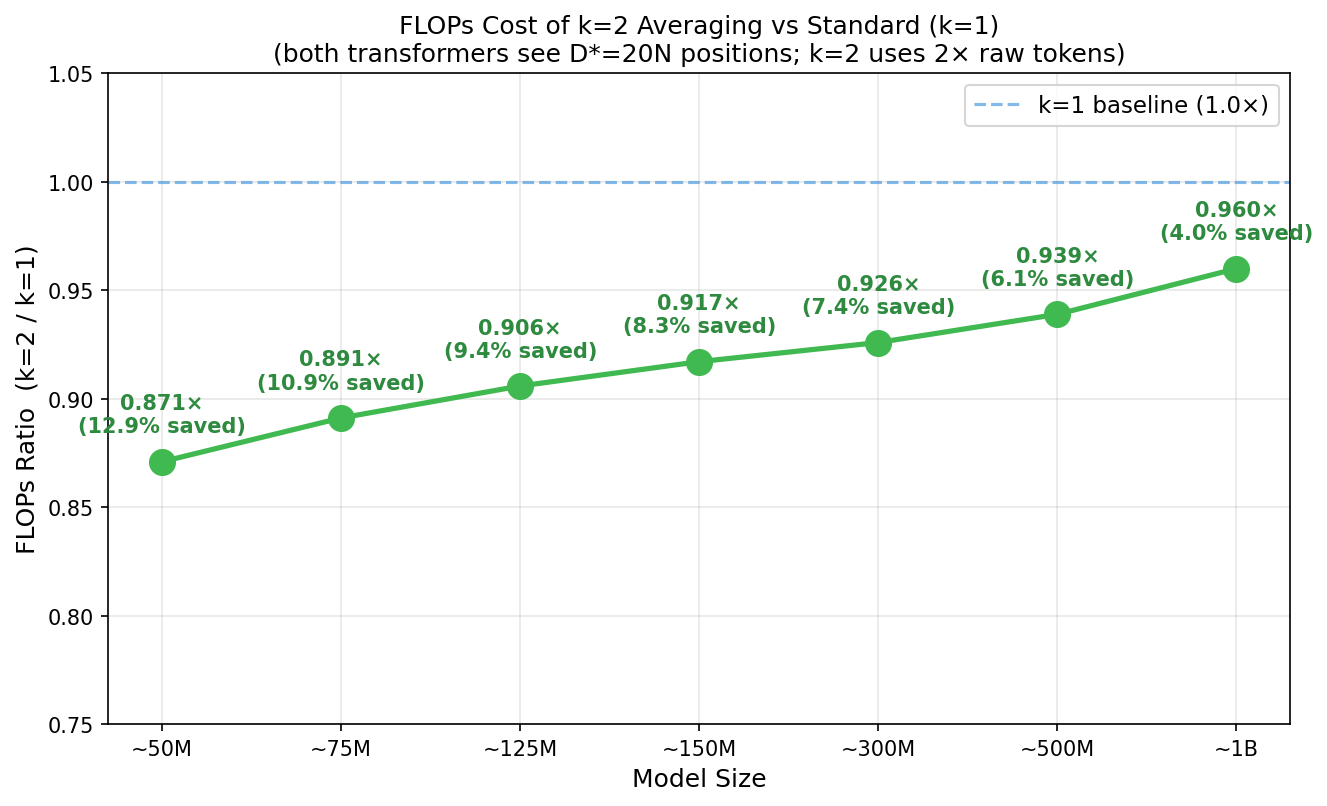
\includegraphics[height=0.52\textheight]{flops_scaling_ratio.png}

  \small At iso-data-multiple, the raw FLOPs saving is only the attention share
  --- and it \bad{shrinks with $d_{\text{model}}$}.
\end{frame}

\begin{frame}{FLOPs picture across scales}
  \centering
  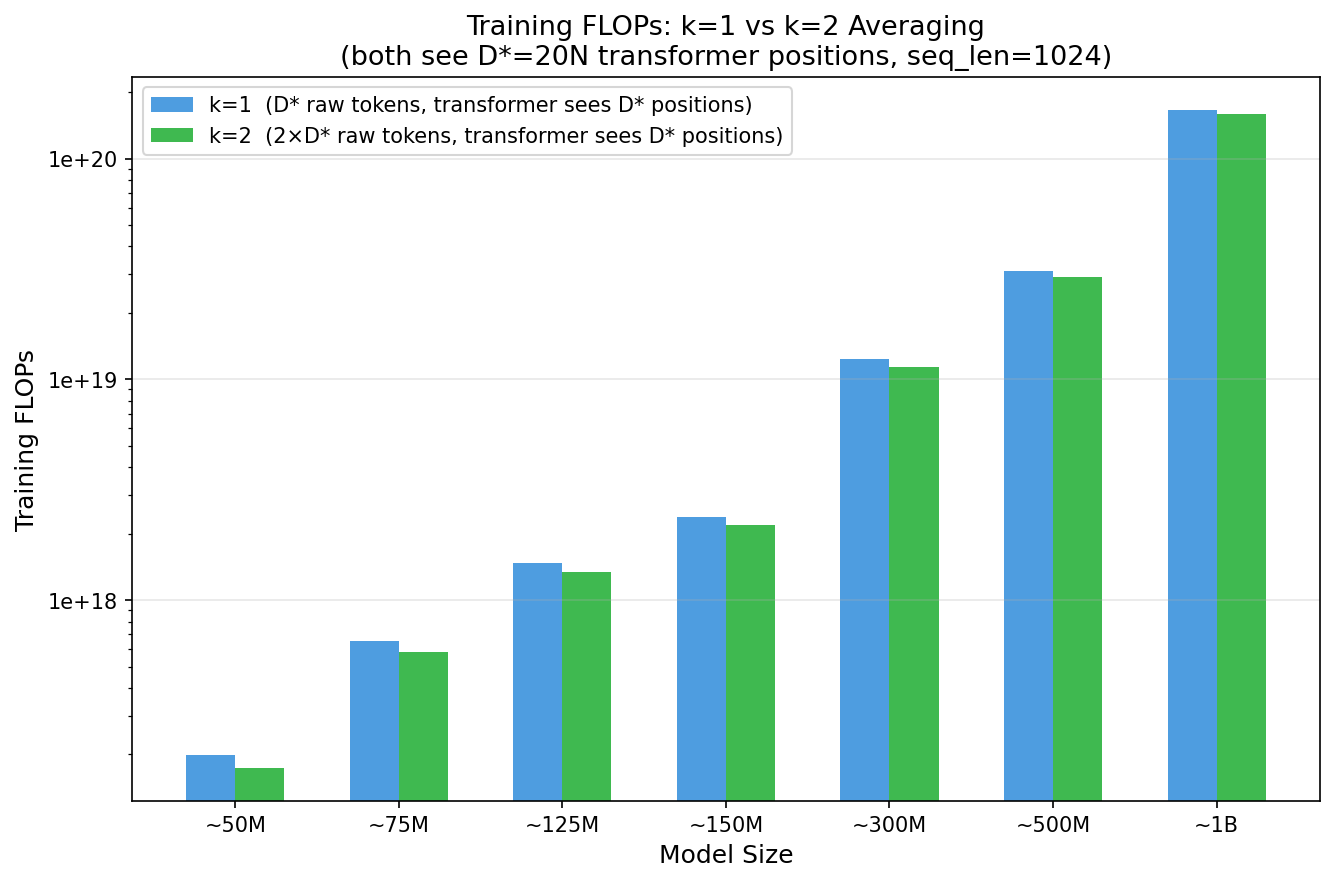
\includegraphics[width=0.49\textwidth]{flops_scaling_absolute.png}\hfill
  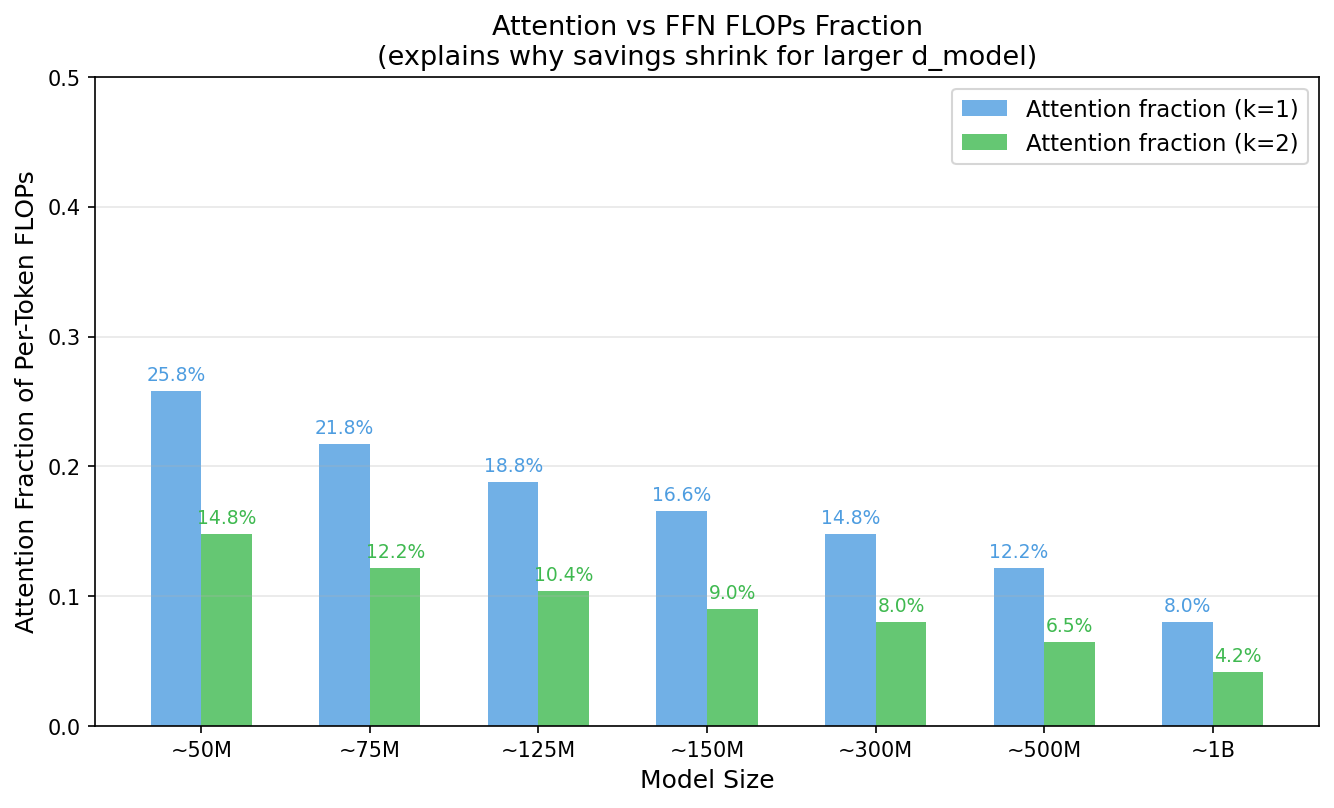
\includegraphics[width=0.49\textwidth]{flops_scaling_attention_fraction.png}

  \vspace{0.4em}
  \begin{alertblock}{Key reframing}
    The arithmetic saving ($4$--$13\%$) is not the story. The story is:
    \textbf{$k{=}2$ embeds $2\times$ the raw data into the same transformer
    budget.} The value of the method is data/context throughput per FLOP, not
    cheaper matmuls.
  \end{alertblock}
\end{frame}

% =====================================================================
\section{Results so far}
% =====================================================================

\begin{frame}{125M: loss vs training FLOPs (iso-FLOPs endpoints)}
  \centering
  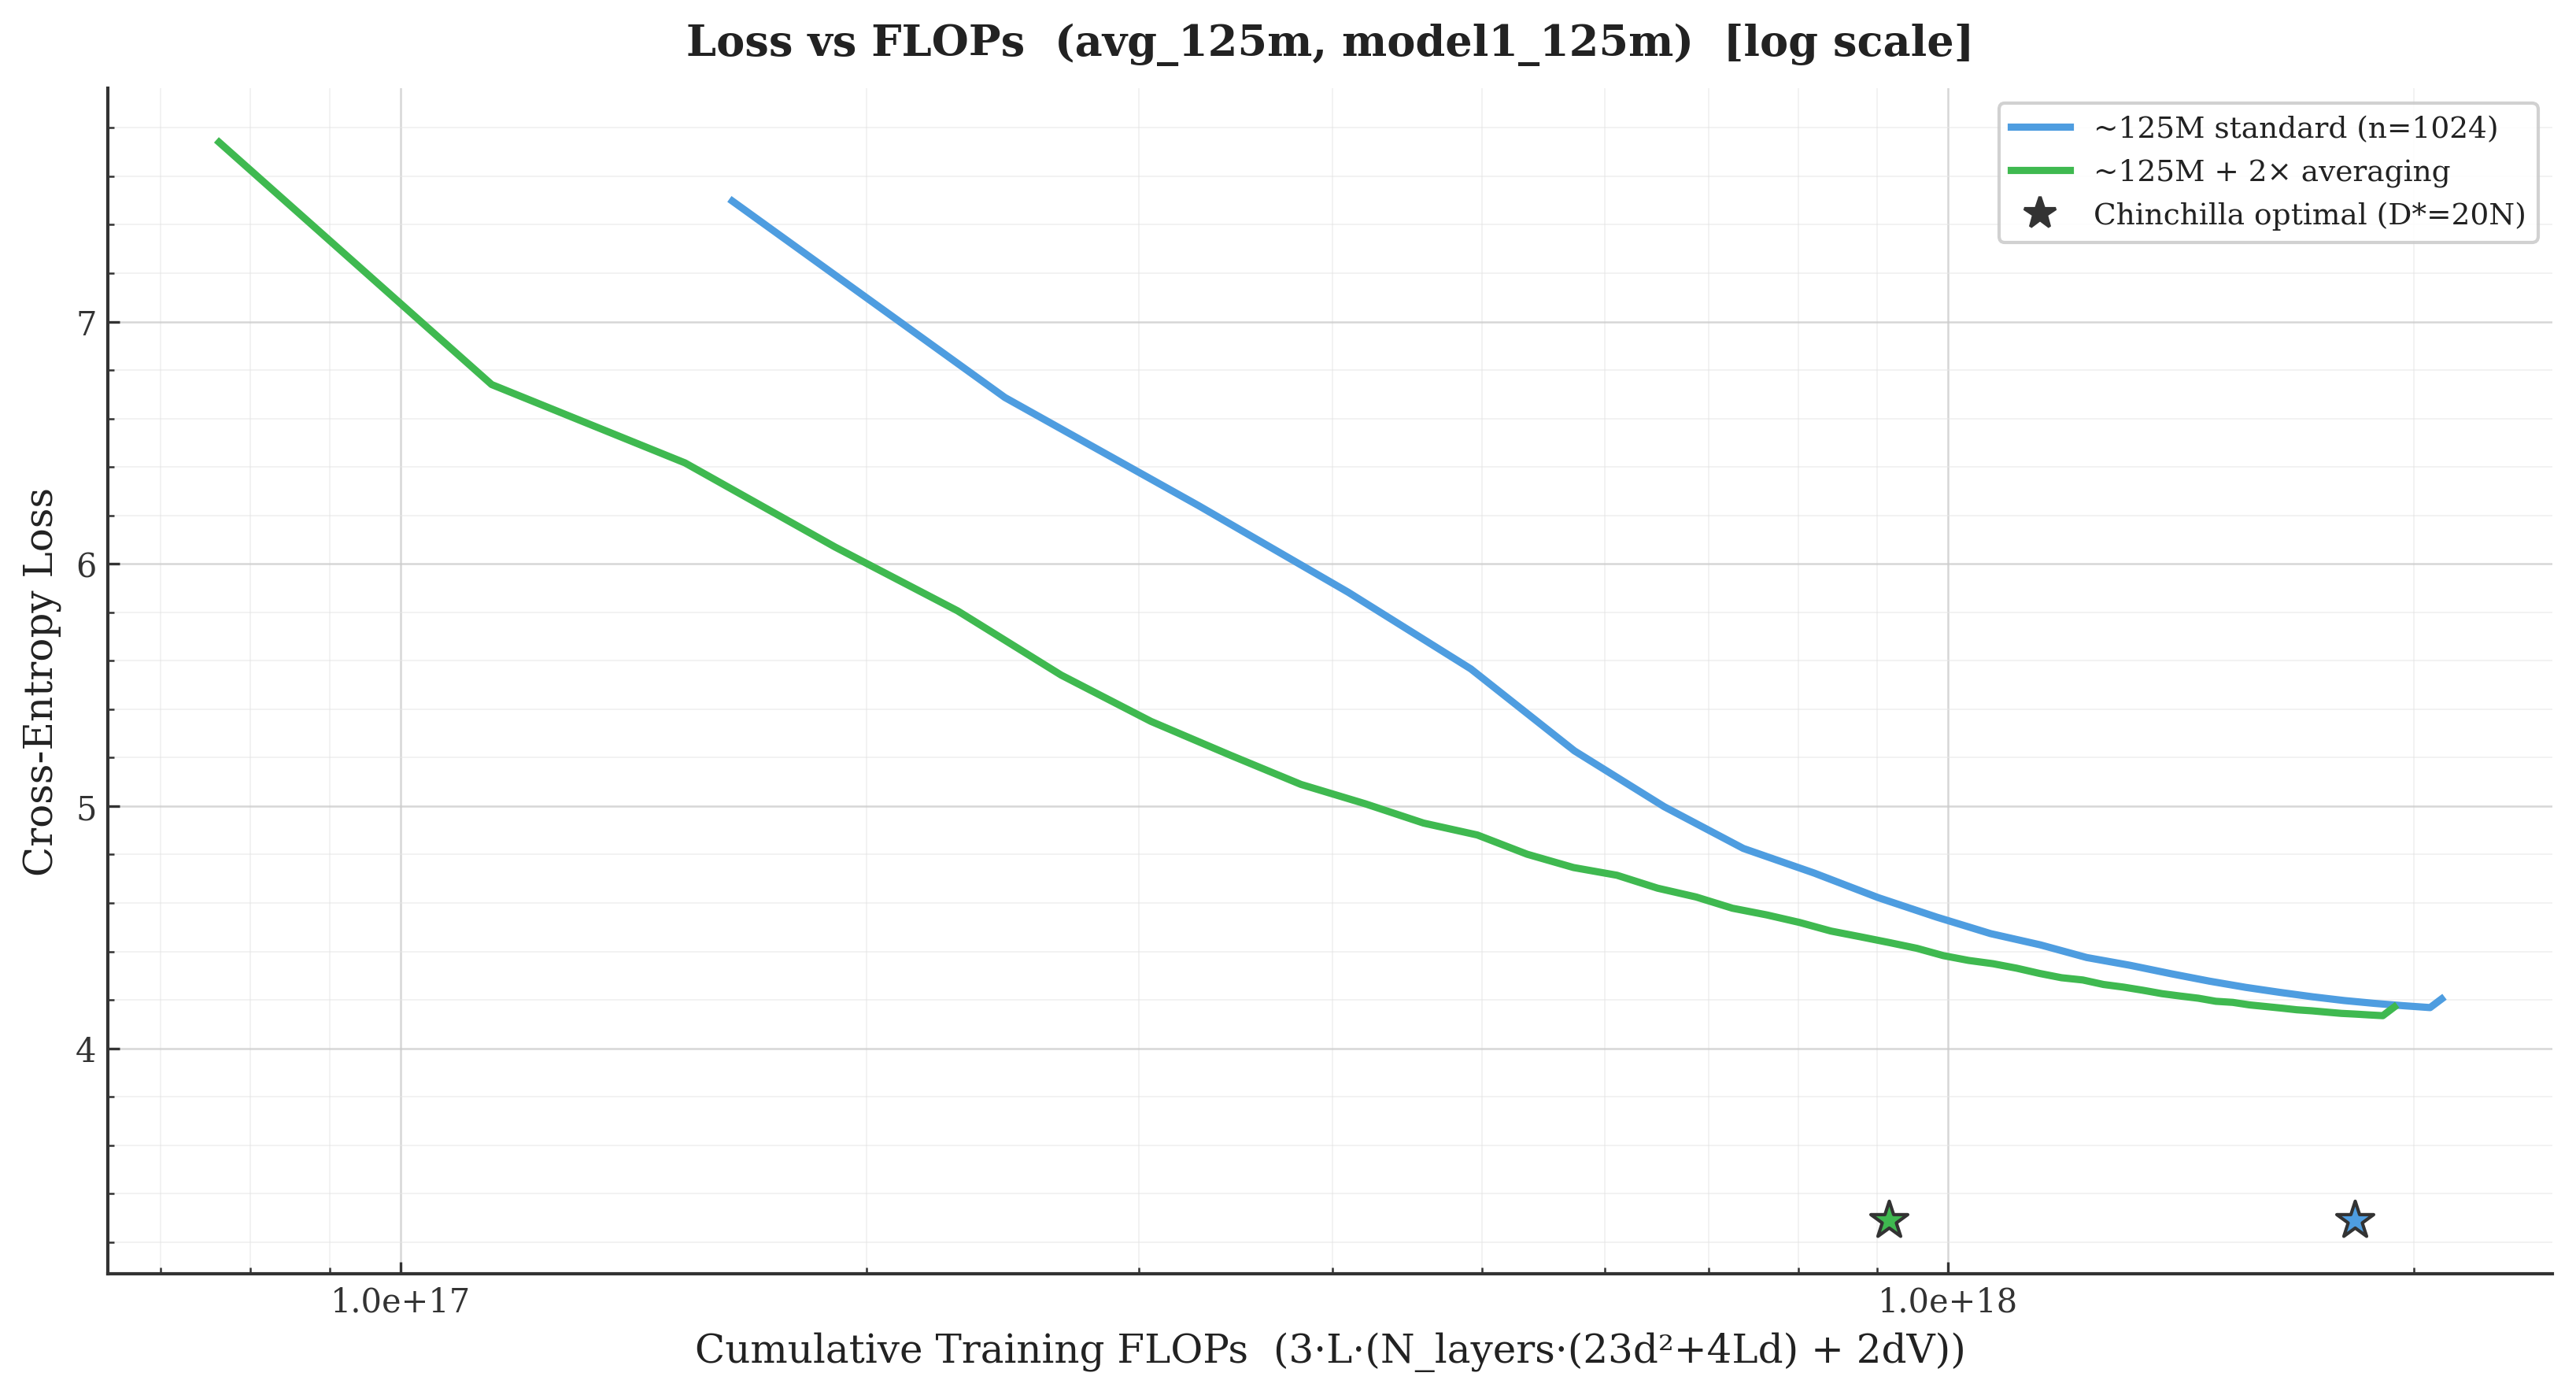
\includegraphics[height=0.72\textheight]{125m_loss_vs_flops_log.png}

  \small $k{=}2$ (green) dominates the baseline over the whole trajectory at
  equal FLOPs.
\end{frame}

\begin{frame}{125M: loss vs raw tokens seen}
  \centering
  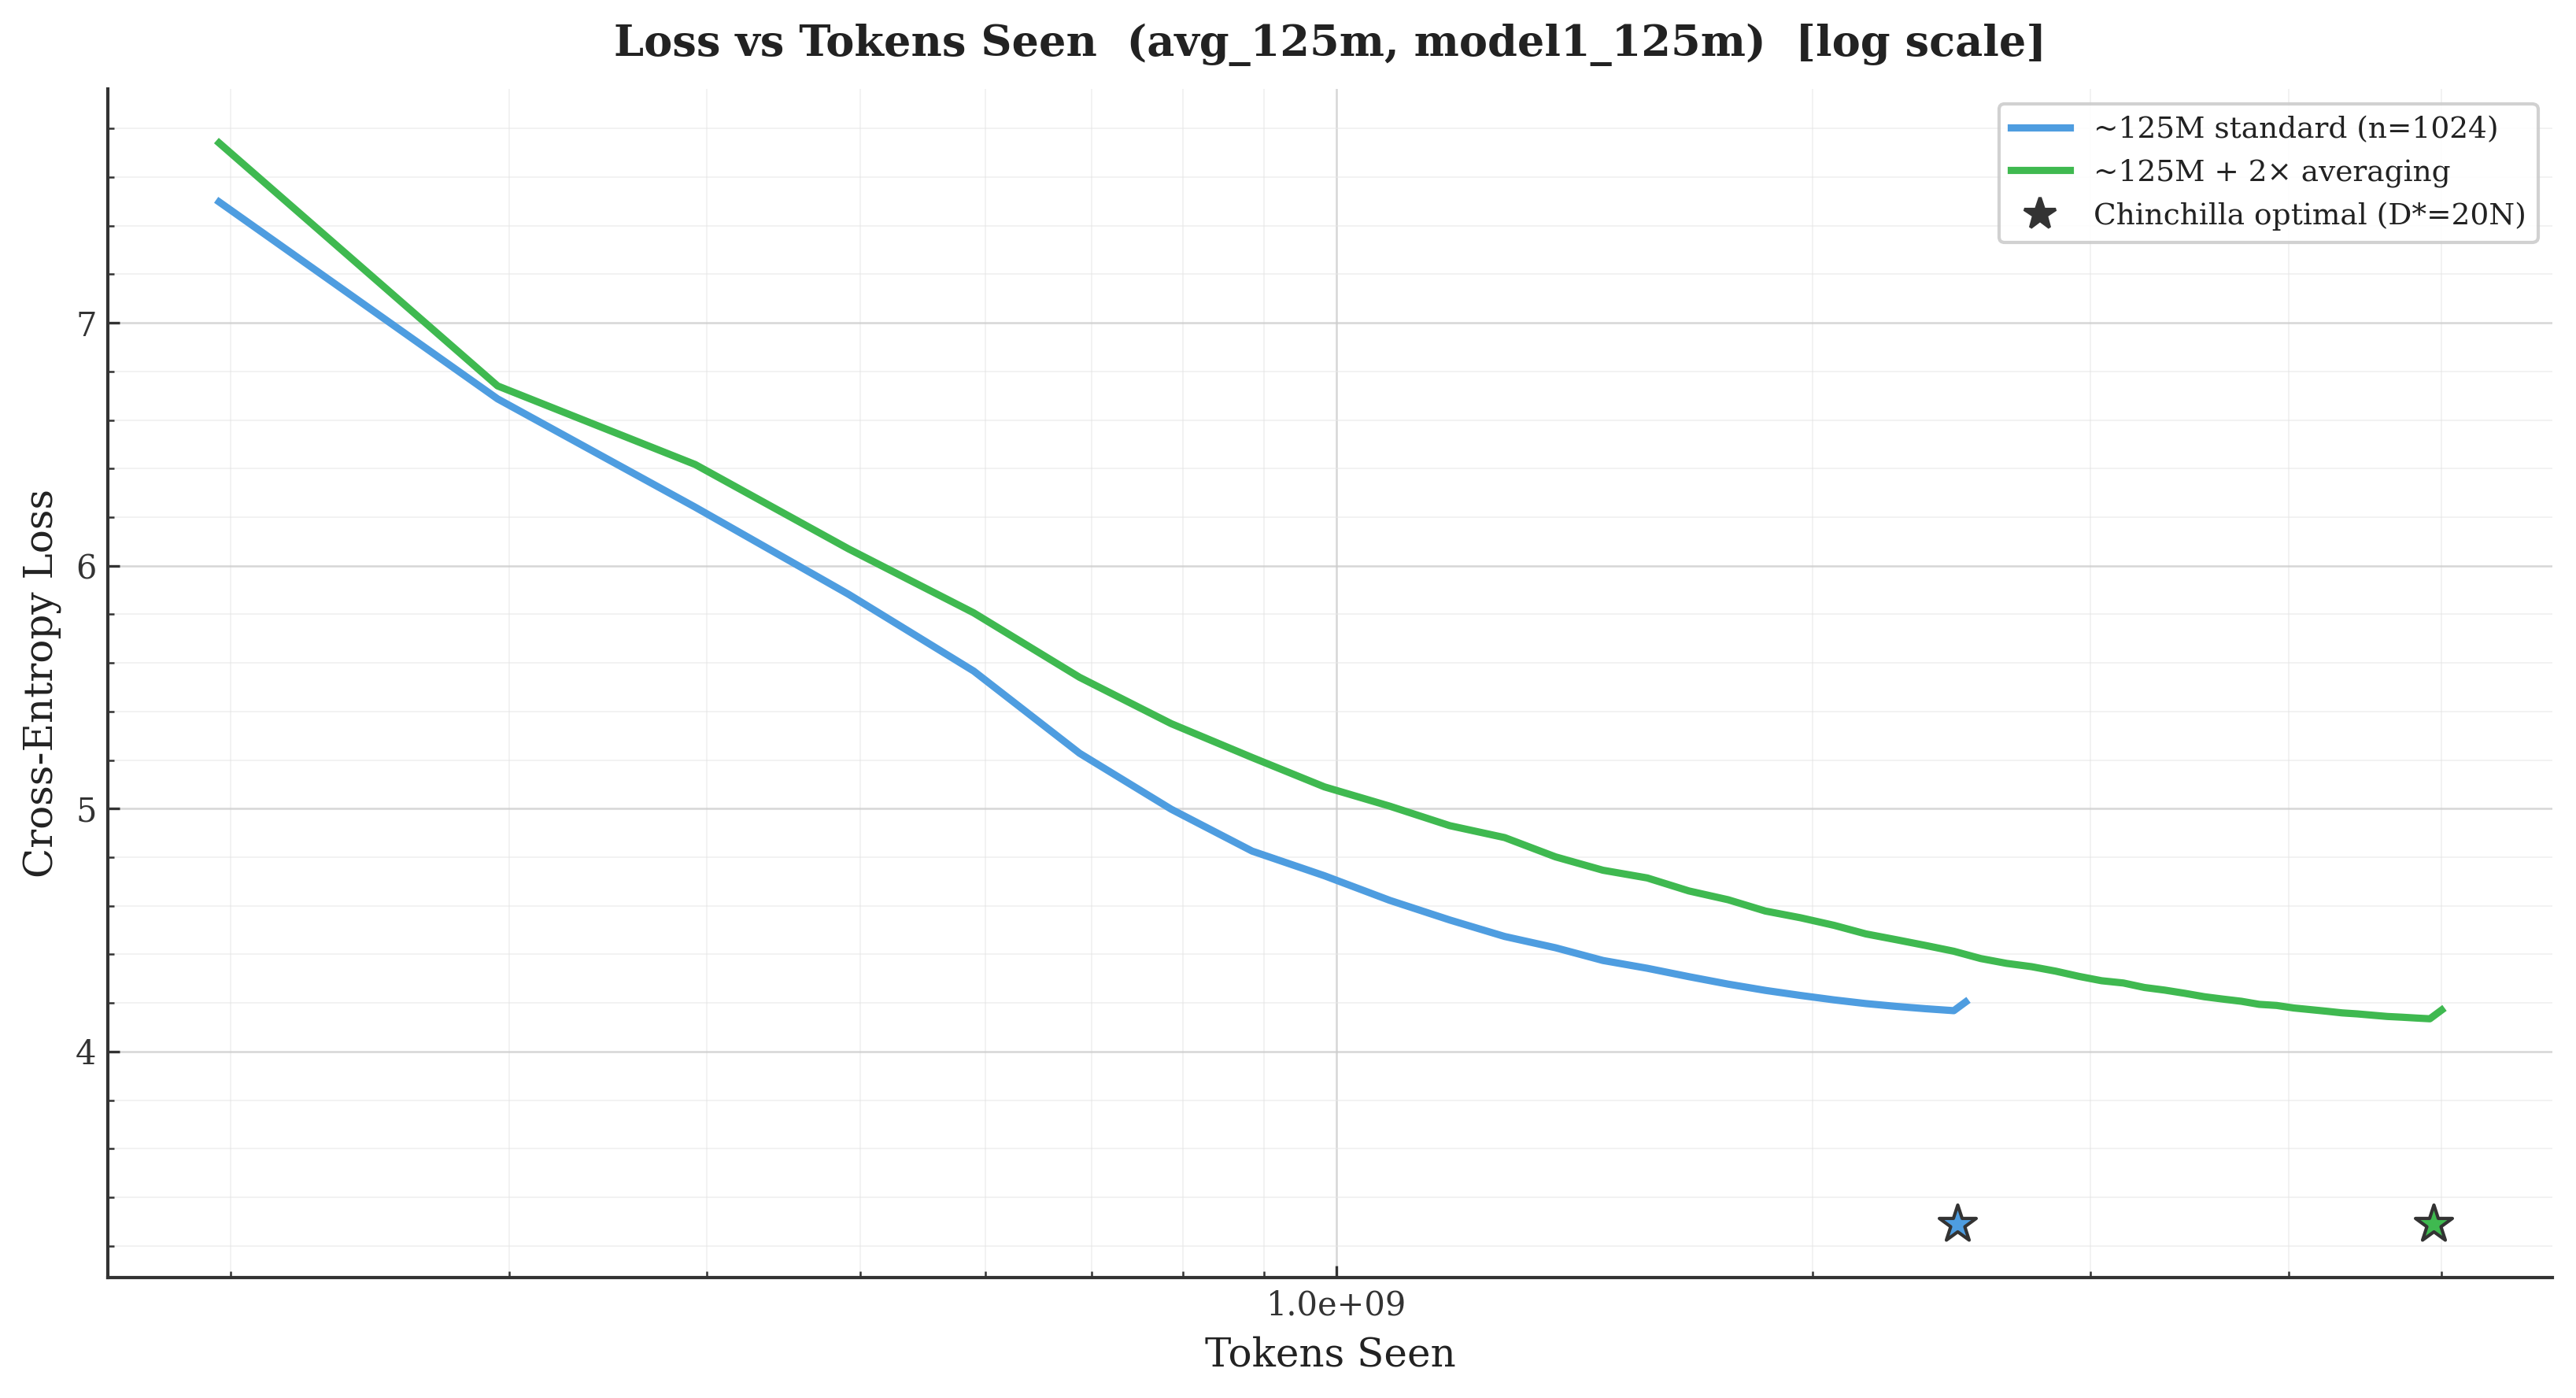
\includegraphics[height=0.72\textheight]{125m_loss_vs_tokens_log.png}

  \small Per raw token the averaged model learns \emph{slightly less} (green
  above blue) --- but each of its tokens costs half the compute, so it wins on
  the FLOPs axis.
\end{frame}

\begin{frame}{Endpoint numbers (training-log eval)}
  \footnotesize
  \centering
  \begin{tabular}{lccccc}
    \toprule
    Run & Raw tokens & Train FLOPs & Final eval & Running eval \\
    \midrule
    125M $k{=}1$ & 2.5B & $1.50\times10^{18}$ & 4.204 & 4.168 \\
    125M $k{=}2$ & 5.0B & $1.36\times10^{18}$ & \good{4.171} & \good{4.135} \\
    250M $k{=}1$ & 5.0B & $6.79\times10^{18}$ & 3.414 & 3.380 \\
    250M $k{=}2$ & 10.0B & $6.29\times10^{18}$ & \good{3.403} & \good{3.362} \\
    \bottomrule
  \end{tabular}

  \vspace{0.3em}
  Two ways to read the same curves:
  \begin{itemize}
    \item \textbf{Equal compute, compare loss (vertical):} at the $k{=}2$
          budget of $1.36\times10^{18}$, baseline is at 4.185 vs
          \good{4.171} --- $k{=}2$ is better while also having spent
          $0.91\times$ the FLOPs at its endpoint
    \item \textbf{Equal loss, compare compute (horizontal):} baseline needs its
          full $1.50\times10^{18}$ to reach 4.204; the $k{=}2$ curve crosses
          4.204 at $1.05\times10^{18}$ $\Rightarrow$
          \good{$\mathbf{1.44\times}$ less compute}.
          (Small vertical gaps $=$ large horizontal gaps: loss curves are very
          flat late in training)
    \item 50M pair, now using the \textbf{matched-protocol $k{=}2$ rerun}
          (4.363 vs baseline 4.437, same tokens/update, both tied):
          \good{$\mathbf{1.58\times}$} saving. The old-protocol $k{=}2$ log
          gave 1.15\texttimes{} for the same comparison --- update schedule
          alone moves the multiplier
    \item 250M pair (full budgets, random-offset training):
          \good{$\mathbf{1.32\times}$} saving by the same reading
    \item Multiplier across scales: $1.58 \to 1.44 \to 1.32 \to$
          \bad{noise floor at 500M} (next section) ---
          \bad{shrinking, not growing}; and all pairs share the
          update-count confound resolved on the next slides
  \end{itemize}
\end{frame}

\begin{frame}{250M pair complete (random-offset training, full budgets)}
  \centering
  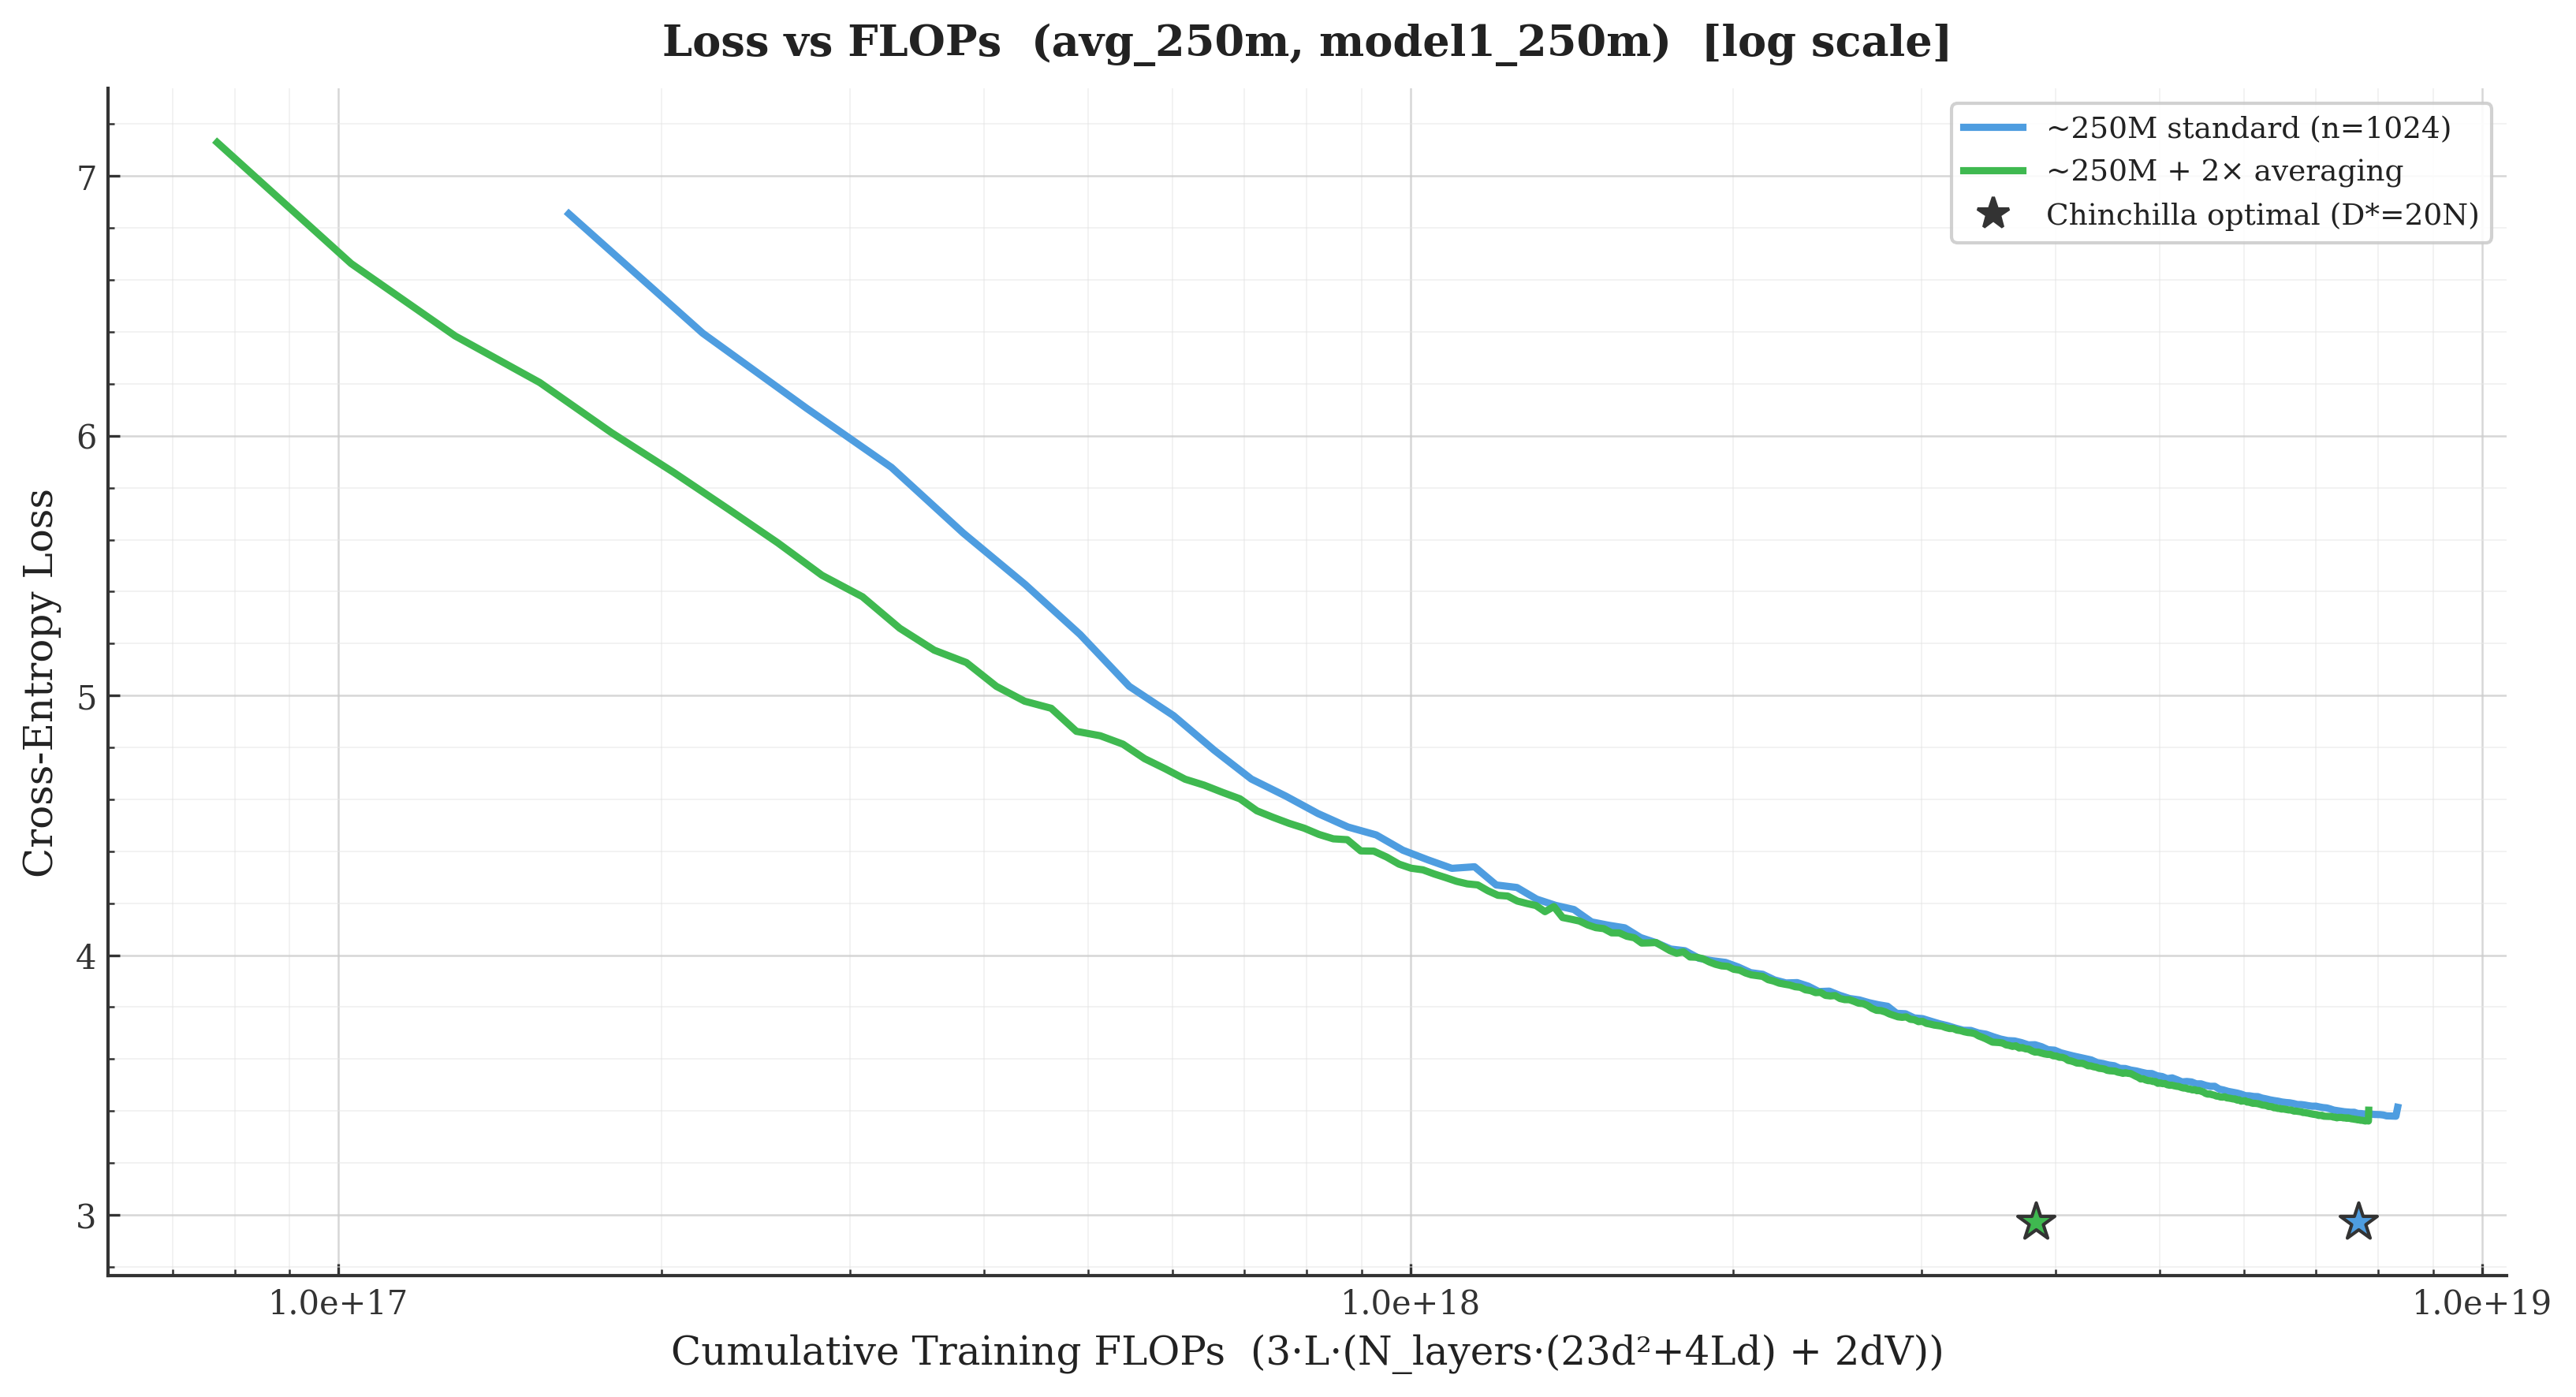
\includegraphics[height=0.5\textheight]{250m_loss_vs_flops_log.png}

  \vspace{0.2em}
  \footnotesize
  \begin{tabular}{lccccc}
    \toprule
    Run & Raw tokens & Train FLOPs & Final eval & Running eval & Saving \\
    \midrule
    250M $k{=}1$ & 5.0B  & $6.79\times10^{18}$ & 3.414 & 3.380 & --- \\
    250M $k{=}2$ & 10.0B & $6.29\times10^{18}$ ($0.93\times$) & \good{3.403} & \good{3.362} &
      \good{$1.32\times$} \\
    \bottomrule
  \end{tabular}

  \vspace{0.3em}
  \raggedright
  \footnotesize Same qualitative picture as 50M/125M: $k{=}2$ ends below the
  baseline at fewer FLOPs. But the equal-loss multiplier keeps shrinking with
  scale, and at iso-FLOPs the $k{=}2$ arm still takes $2\times$ the optimizer
  updates (both arms ran 32{,}768 raw tokens/update) --- the confound the next
  slide isolates.
\end{frame}

\begin{frame}{500M pair complete: the decay reaches the noise floor}
  \centering
  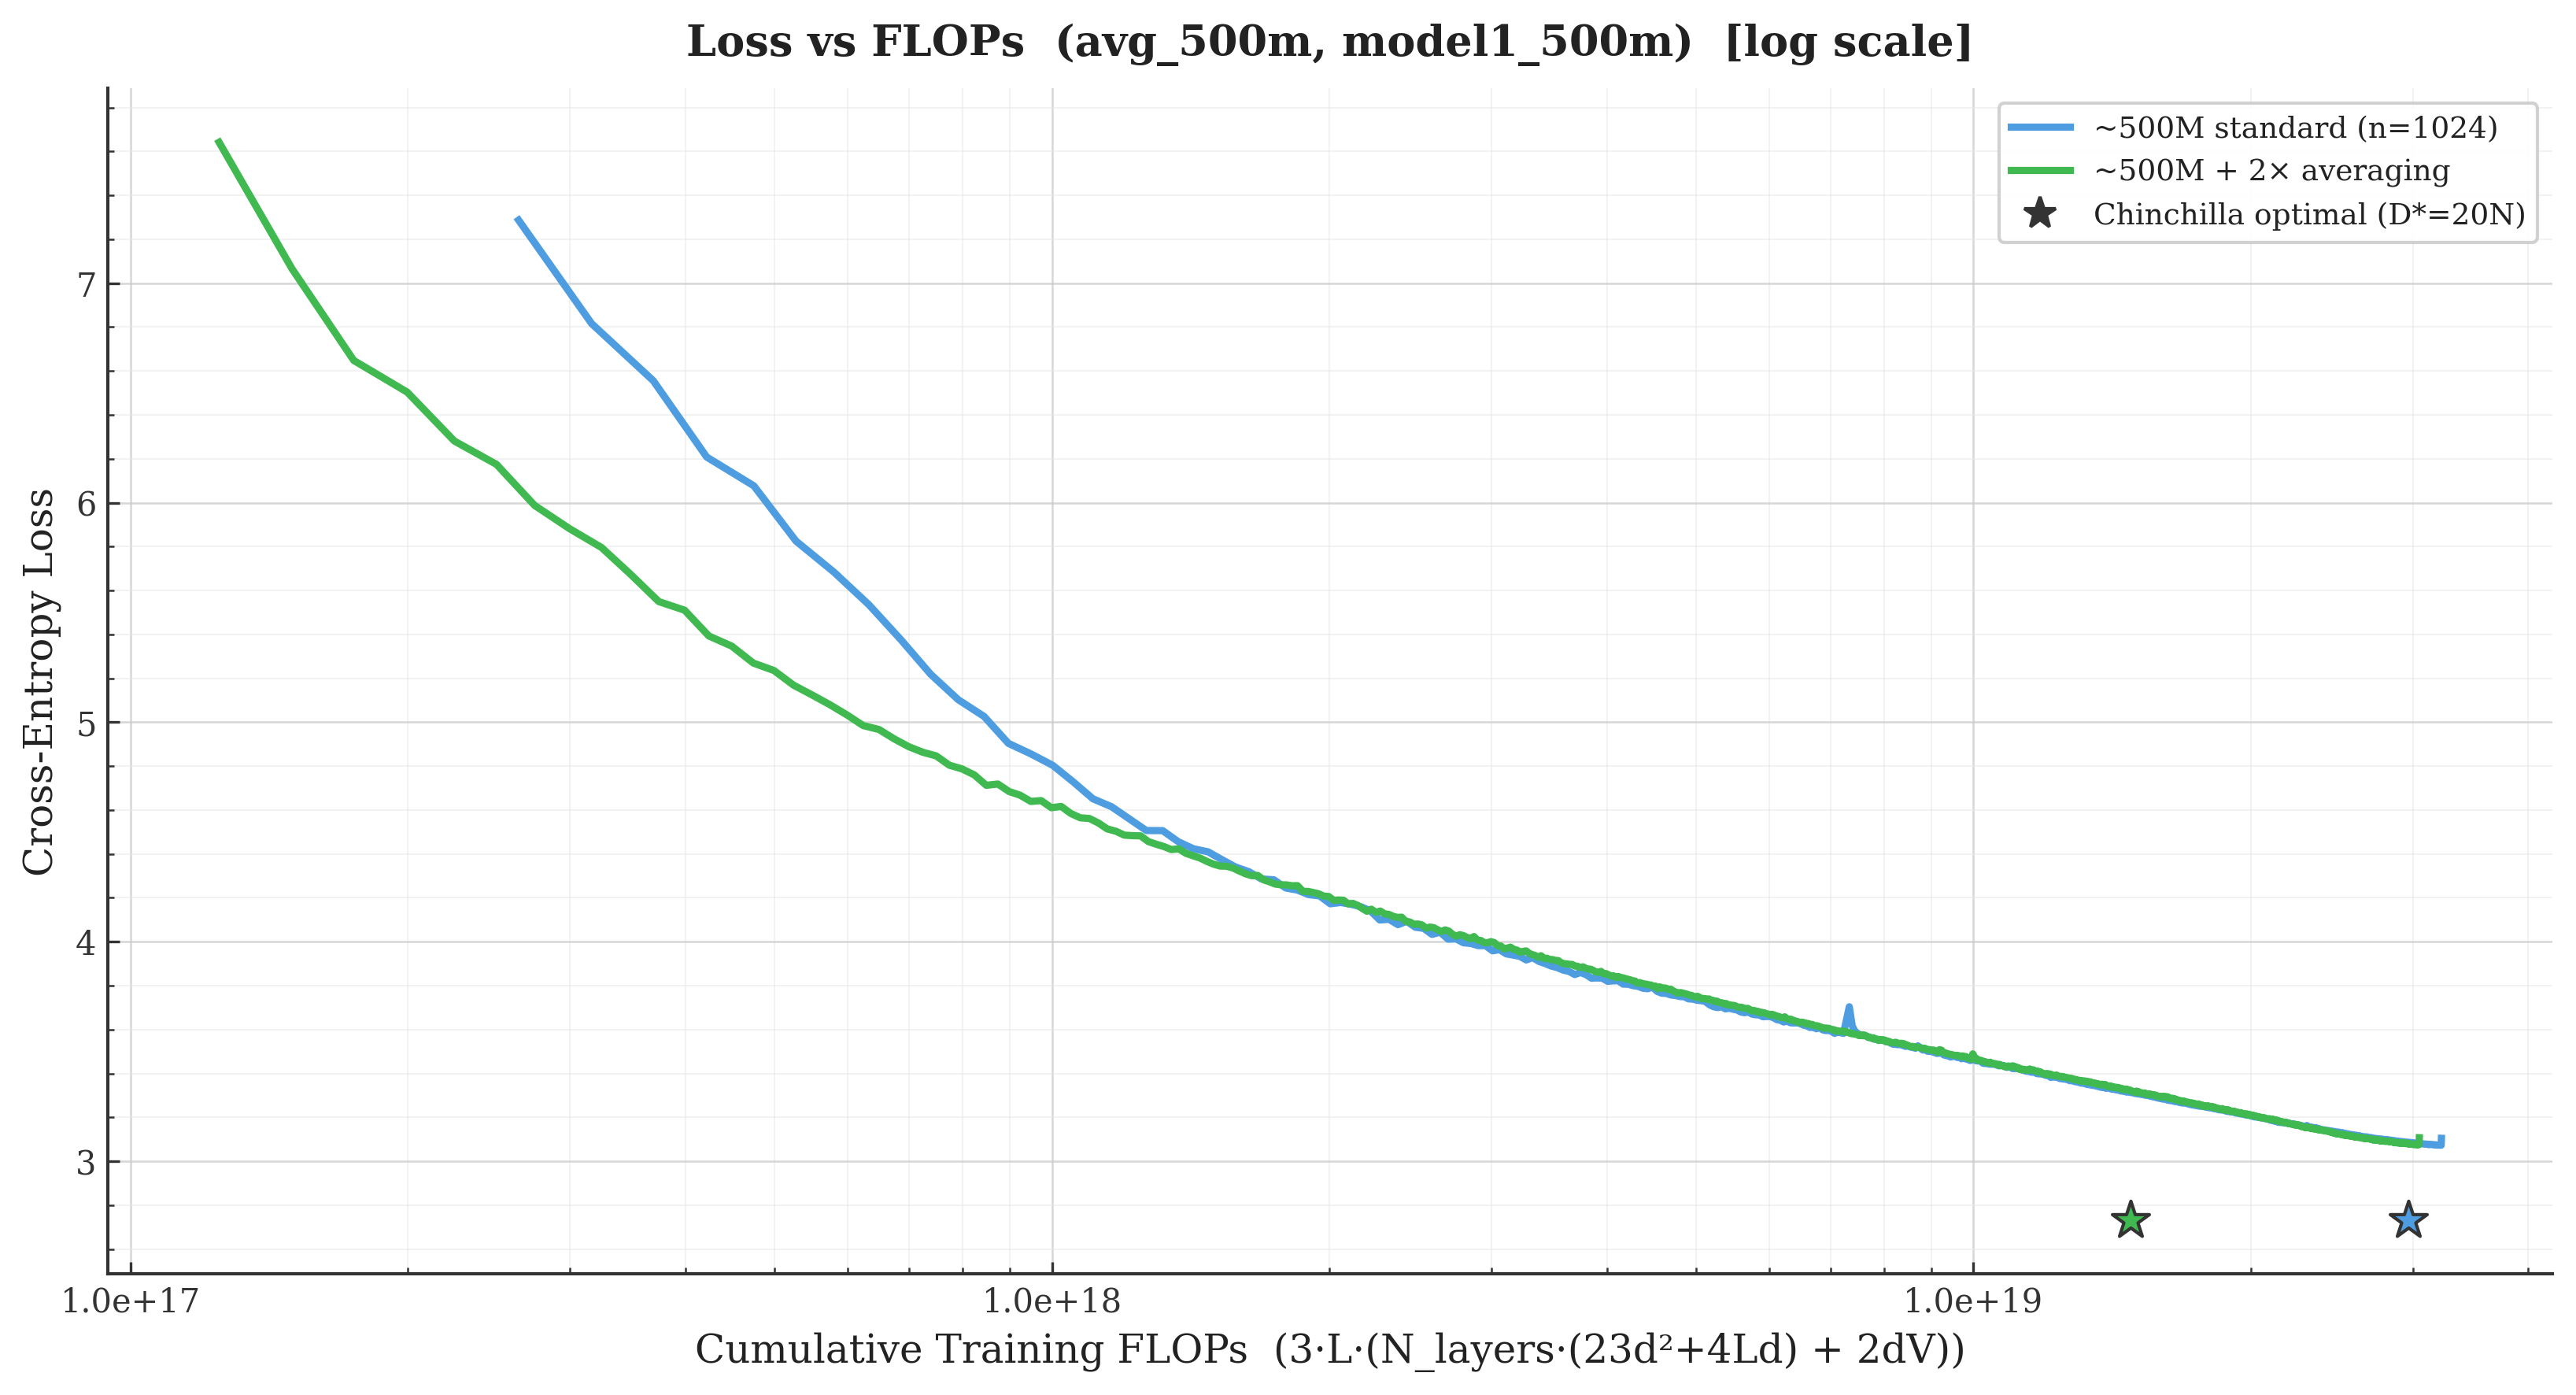
\includegraphics[height=0.44\textheight]{500m_loss_vs_flops_log.png}

  \vspace{0.15em}
  \footnotesize
  \begin{tabular}{lcccc}
    \toprule
    Run & Raw tokens & Train FLOPs & Full-position eval \\
    \midrule
    500M $k{=}1$ & 10.0B & $3.22\times10^{19}$ & 3.073 \\
    500M $k{=}2$ & 20.0B & $3.05\times10^{19}$ ($0.946\times$) & \good{3.071} \\
    \bottomrule
  \end{tabular}

  \vspace{0.2em}
  \raggedright
  \footnotesize \textbf{The sign flips depending on which metric you read.}
  Native loss now slightly \emph{favors the baseline} ($-0.003$ nats); the
  full-position metric (comparable across $k$) still favors averaging
  ($+0.003$ nats). Both are an order of magnitude below the $0.070$-nat
  shift the training protocol alone caused at 50M, with zero seed replicates
  to bound noise at this scale --- not a clean win or a clean loss.

  \vspace{0.15em}
  \tiny FLOPs include the output projection ($2dV$); the 125M/250M numbers on
  earlier slides predate that fix and are not directly comparable to this
  table until reconciled.
\end{frame}

\begin{frame}{What the 500M point means: the gap shrinks but holds}
  \footnotesize
  On the \textbf{full-position eval} (the comparable metric across $k$),
  averaging still wins at every scale where we have measured it:

  \vspace{0.2em}
  \centering
  \begin{tabular}{lccc}
    \toprule
    Scale & Native gap ($k{=}1 - k{=}2$) & Full-position gap & Status \\
    \midrule
    50M   & $0.074$  & (not yet measured) & \\
    125M  & $0.033$  & \good{$0.037$}     & \good{$k{=}2$ wins} \\
    250M  & $0.011$  & (not yet measured)  & \\
    500M  & $-0.003$ & \good{$0.003$}     & \good{$k{=}2$ still wins} \\
    \bottomrule
  \end{tabular}

  \vspace{0.25em}
  \raggedright
  \begin{itemize}
    \item On the native metric the gap crossed zero at 500M ($-0.003$),
          but native loss is not comparable across $k$ --- this is the
          metric we declared invalid for cross-$k$ comparison
    \item On the full-position metric, \good{averaging still wins at 500M}
          ($+0.003$ nats), though the margin is tiny and shrinking
          ($0.037 \to 0.003$ from 125M to 500M)
    \item The gap is small enough to be within single-seed noise (we
          have zero replicates at this scale). Seed replicates at 500M
          would settle whether this is a real residual win or noise
    \item Missing: full-position eval at 50M and 250M (currently only
          native gaps; rescore queued)
  \end{itemize}

  \vspace{0.15em}
  \begin{alertblock}{Reading}
    The decay trend is real: the advantage shrinks with scale. But on the
    comparable metric it has \emph{not} crossed zero yet. Whether it
    reaches zero at 1B or stabilizes at a small positive value is the open
    question.
  \end{alertblock}
\end{frame}

\begin{frame}{Update-count control: the 50M gain does not survive}
  \centering
  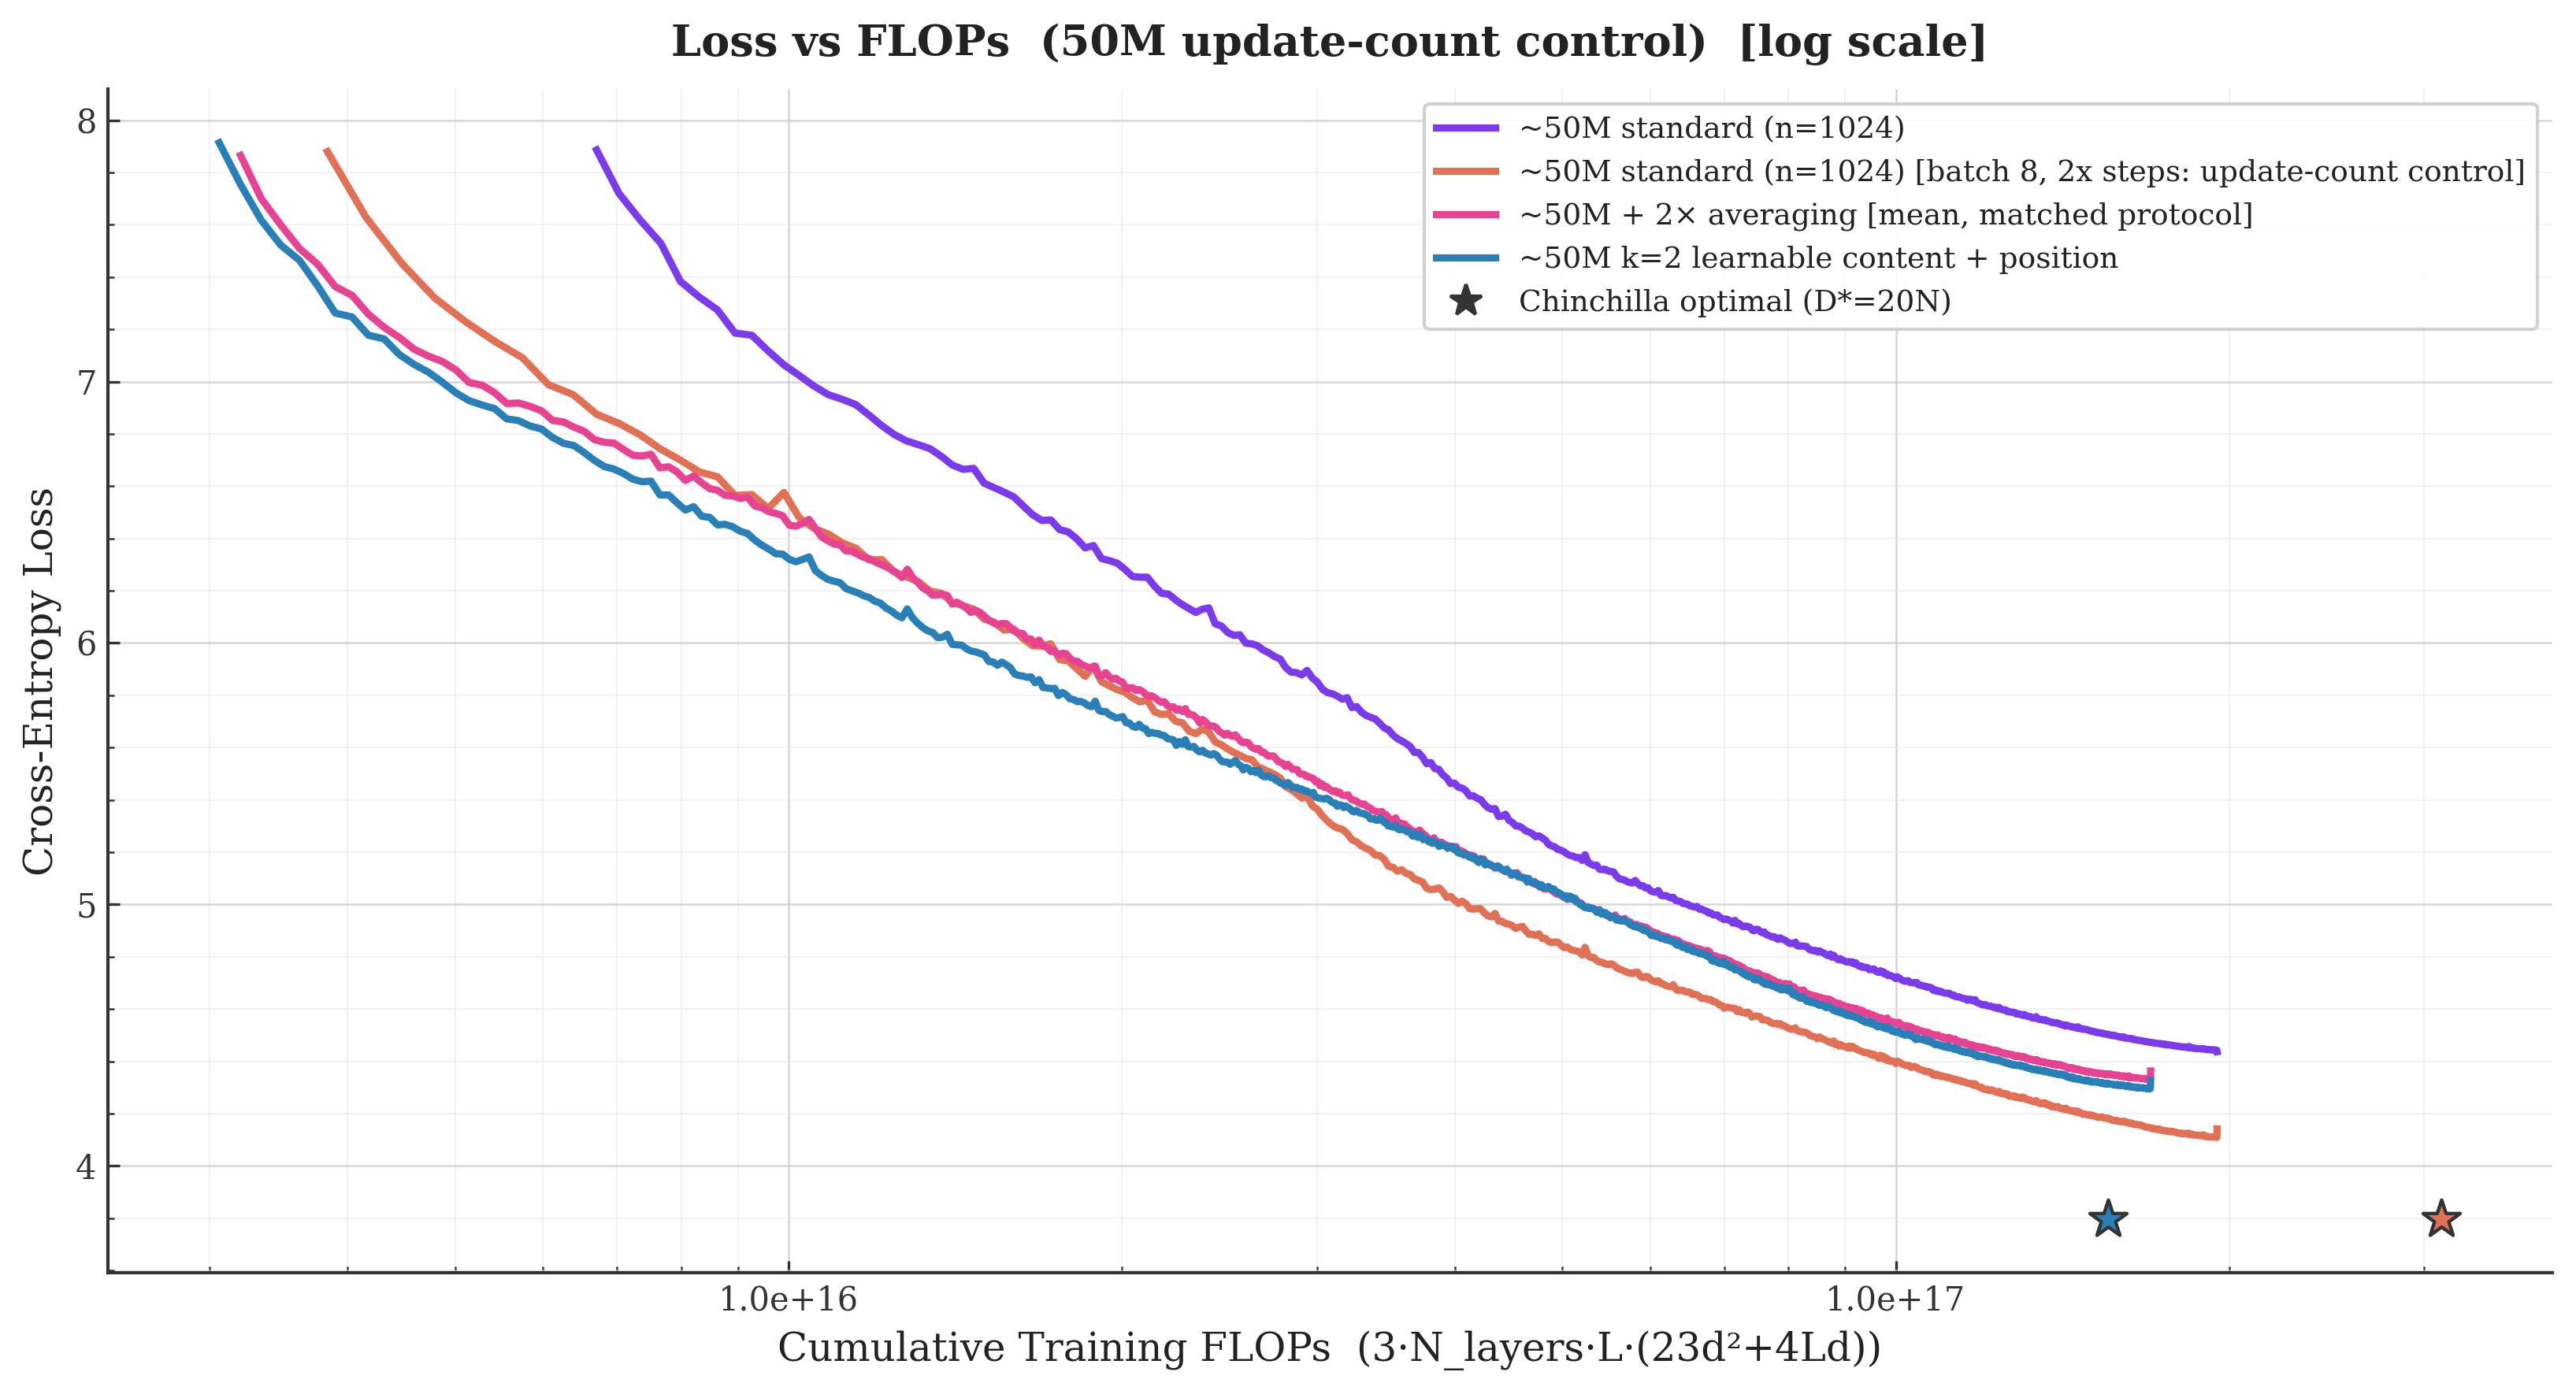
\includegraphics[height=0.47\textheight]{50m_update_ctrl_loss_vs_flops_log.png}

  \vspace{0.2em}
  \footnotesize
  \begin{tabular}{lcccc}
    \toprule
    Run (50M) & Raw tokens & Updates & Train FLOPs & Final eval \\
    \midrule
    $k{=}1$ baseline (batch 16) & 1B & 61k & $1.95\times10^{17}$ & 4.437 \\
    $k{=}2$ mean, matched & 2B & 122k & $1.70\times10^{17}$ & 4.363 \\
    $k{=}2$ learnable+pos & 2B & 122k & $1.70\times10^{17}$ & 4.326 \\
    \textbf{$k{=}1$ control (batch 8)} & 1B & \textbf{122k} &
      $1.95\times10^{17}$ & \good{\textbf{4.142}} \\
    \bottomrule
  \end{tabular}

  \vspace{0.3em}
  \raggedright
  \footnotesize The control is the baseline with half the batch: same 1B raw
  tokens and FLOPs, but the \emph{same 122k updates and the same 8{,}192
  transformer positions per update as the $k{=}2$ arms}. Only the input
  resolution differs.
\end{frame}

\begin{frame}{Update-count control: readings}
  \footnotesize
  \begin{itemize}
    \item \bad{The control beats every $k{=}2$ variant}: 4.142 vs 4.326 for
          the best pooling rule. It reaches $k{=}2$ mean's final loss (4.363)
          at $1.06\times10^{17}$ FLOPs --- $0.62\times$ of what $k{=}2$
          spent --- and learnable+pos's 4.326 at 59\% of its own budget
    \item \bad{Update schedule explains more than the whole 50M headline}:
          batch $16 \to 8$ at identical data and FLOPs moves the baseline by
          $-0.295$ nats; the $k{=}2$ edge over the batch-16 baseline was only
          $-0.074$
    \item At 61k updates (same count as the batch-16 baseline, but only 0.5B
          tokens and half the FLOPs), the control has \emph{already} matched
          the baseline's final loss (4.420 vs 4.443) --- at this scale, loss
          tracks update count far more than data seen
    \item Metric caveat: these are native losses (cross-$k$), but at 125M the
          native and full-position readings differed by $\sim$0.005 nats ---
          a 0.22-nat gap will not flip
  \end{itemize}

  \vspace{0.3em}
  \begin{alertblock}{Implication}
    At 50M, with updates and positions matched, \textbf{raw tokens beat
    averaged tokens}. The iso-FLOPs training-efficiency claim now rests
    entirely on whether this control repeats at 125M/250M --- run it there
    before any 500M/1B spend. (Open question in averaging's favor: does
    $k{=}2$ also improve with batch 8? Both arms deserve the tuned setting.)
  \end{alertblock}
\end{frame}

\begin{frame}{New experiment: is it a data effect or a context effect?}
  Two ways to deploy $k$-averaging at a fixed FLOP budget:

  \vspace{0.4em}
  \centering
  \small
  \begin{tabular}{lcccc}
    \toprule
    & seq\_len (raw) & Transformer len & Raw context & Tokens trained \\
    \midrule
    $k{=}1$ baseline      & 1024 & 1024 & 1024 & 1B \\
    \textbf{Config A}: $k{=}2$, same seq   & 1024 & 512  & 1024 & 2B \\
    \textbf{Config B}: $k{=}2$, same $L$   & 2048 & 1024 & \acc{2048} & 2B \\
    \textbf{Config B}: $k{=}4$, same $L$   & 4096 & 1024 & \acc{4096} & 4B \\
    $k{=}1$ full attention & 2048 & \bad{2048} & \acc{2048} & 1B \\
    \bottomrule
  \end{tabular}

  \vspace{0.8em}
  \raggedright
  \begin{itemize}
    \item Config A pockets the compute saving (shorter transformer sequences)
    \item Config B spends it on \emph{extended raw context} at the same
          transformer length --- ``double context for free''
    \item Per raw token, Config B costs exactly $1/k$ of baseline
          $\Rightarrow$ iso-FLOPs at $k\times$ tokens, by construction
    \item $k{=}1$ full attention: the \emph{traditional} way to get 2048
          context --- costs $1.26\times$ baseline per token ($L{=}2048$
          attention)
  \end{itemize}
\end{frame}

\begin{frame}{Result: extended context \bad{loses} at $\sim$iso-FLOPs (50M)}
  \centering
  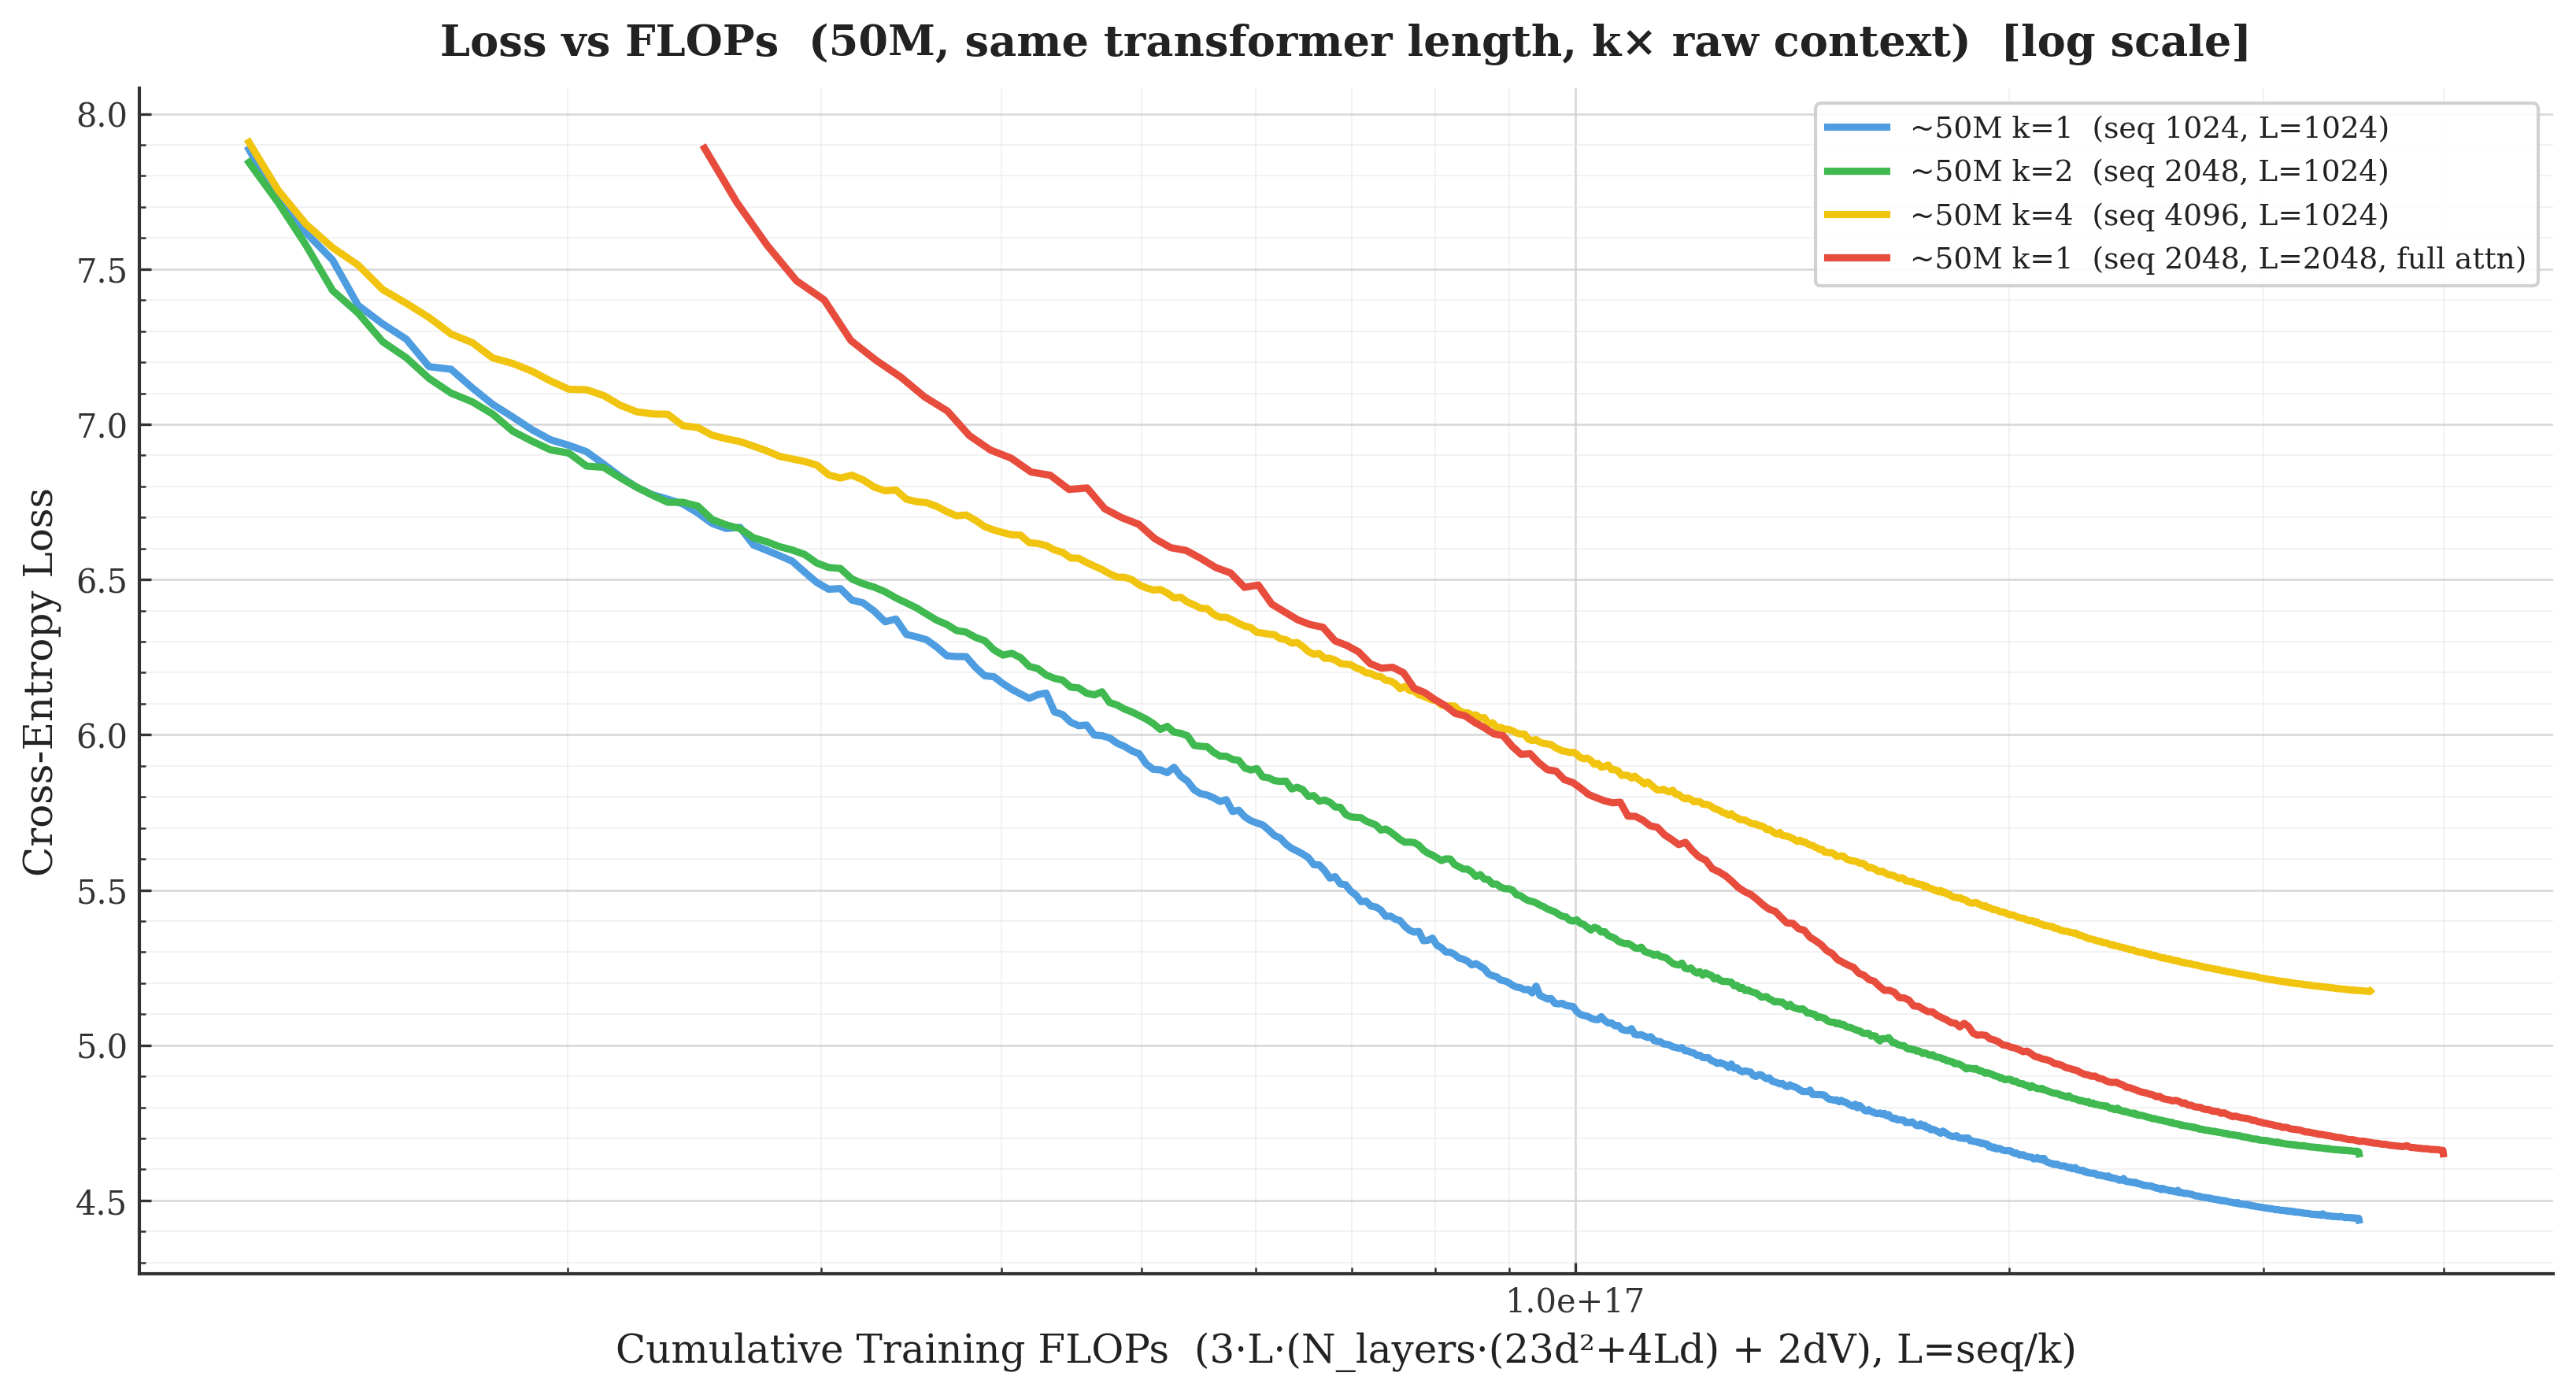
\includegraphics[height=0.54\textheight]{50m_kx_ctx_loss_vs_flops_log.png}

  \vspace{0.2em}
  \small
  \begin{tabular}{lcccc}
    \toprule
    Run & Raw tokens & FLOPs & Final eval & vs baseline \\
    \midrule
    $k{=}1$, seq 1024            & 1.00B & $1.95\times10^{17}$ & \good{4.437} & --- \\
    $k{=}2$, seq 2048            & 2.00B & $1.95\times10^{17}$ & 4.650 & \bad{$+0.213$} \\
    $k{=}1$, seq 2048 (full attn) & 1.00B & $2.45\times10^{17}$ & 4.651 & \bad{$+0.214$} \\
    $k{=}4$, seq 4096            & 4.07B & $1.99\times10^{17}$ & 5.174 & \bad{$+0.739$} \\
    \bottomrule
  \end{tabular}
\end{frame}

\begin{frame}{Context-for-context: averaging \good{beats} full attention}
  Both 2048-raw-context arms land at (almost eerily) \textbf{identical final
  loss} --- at very different cost:

  \vspace{0.5em}
  \centering
  \begin{tabular}{lcccc}
    \toprule
    2048-context model & Final eval & FLOPs & KV cache & Data seen \\
    \midrule
    $k{=}2$ averaging ($L{=}1024$)   & \good{4.6503} & \good{$1.95\times10^{17}$} & \good{$\tfrac12$} & 2B \\
    $k{=}1$ full attn ($L{=}2048$)   & 4.6505 & $2.45\times10^{17}$ & $1$ & 1B \\
    \bottomrule
  \end{tabular}

  \vspace{0.8em}
  \raggedright
  \begin{itemize}
    \item Averaging reaches full attention's final loss with
          \good{$\mathbf{1.26\times}$ less compute}; at averaging's budget,
          full attention is still at 4.727
    \item Plus half the KV cache and attention cost at inference for the same
          raw context
  \end{itemize}

  \vspace{0.4em}
  \begin{block}{Two takeaways, one experiment}
    \textbf{(1)} If you want longer raw context, averaging is a strictly
    cheaper way to get it than widening the attention window.
    \textbf{(2)} But on packed FineWeb at 50M, context beyond 1024 hurts
    \emph{by either method} ($+0.21$ nats) --- the failure is the data/scale,
    not the averaging.
  \end{block}
\end{frame}

\begin{frame}{The decomposition: cheaper tokens, not more context}
  \footnotesize
  Same model, same $k{=}2$, same 2B raw tokens --- only where the compute goes
  differs:

  \vspace{0.4em}
  \centering
  \begin{tabular}{lccc}
    \toprule
    & Final eval loss & FLOPs vs baseline & Outcome \\
    \midrule
    Config A ($k{=}2$, seq 1024) & \good{4.363} & $0.87\times$ &
      \good{wins ($1.58\times$ saving)} \\
    Config B ($k{=}2$, seq 2048) & \bad{4.650} & $1.00\times$ &
      \bad{loses; baseline is $1.72\times$ cheaper} \\
    \bottomrule
  \end{tabular}

  \vspace{0.2em}
  \scriptsize Config A value is the matched-protocol rerun (16k
  tokens/update, 122k steps); Config B ran at 32k tokens/update (61k steps,
  same update count as the baseline).

  \vspace{0.4em}
  \raggedright
  \begin{block}{Interpretation}
    The benefit of token averaging is \textbf{data-per-FLOP, not context}.
    Extended raw context does not pay for itself at this scale ---
    \emph{by any method}:
    \begin{itemize}
      \item The $k{=}1$ full-attention control at 2048 context is equally bad
            ($+0.21$ nats) at $1.26\times$ the cost $\Rightarrow$ the failure
            is the data/scale, not averaging
      \item FineWeb docs are mostly $<$1024 tokens; packing crosses document
            boundaries unmasked $\Rightarrow$ context beyond 1024 is largely
            other documents' text
      \item Degradation compounds with $k$ ($+0.21 \to +0.74$ nats), consistent
            with patch-size findings in prior work
    \end{itemize}
  \end{block}

  \vspace{0.2em}
  \scriptsize Caveat before generalizing: needs a loss-vs-position check and a
  long-document dataset (PG19 / code) to rule context in or out at scale.
\end{frame}

% =====================================================================
\section{What went wrong along the way}
% =====================================================================

\begin{frame}{Detours and bugs (and what they taught us)}
  \begin{enumerate}
    \item \bad{RoPE bug} in early runs --- invalidated the first tied-embedding
          and several old $k$-sweep results. Old logs quarantined; only
          post-fix runs are used.
    \item \bad{50M $k{=}1$ baseline instability} --- the original run ended
          $\sim$1 nat too high after an early loss explosion.
          \good{Rerun completed:} clean baseline now ends at 4.437, consistent
          with the 125M scaling pattern. (All runs show a large transient init
          loss that self-recovers by step $\sim$2000 --- an init artifact,
          clipped in plots.)
    \item \acc{The ``seq\_len bug'' that became the design} --- $k{=}2$ was
          accidentally trained with the same raw \texttt{seq\_len}=1024 as
          $k{=}1$ (not 2048). This turned out to be the \emph{cleaner} control:
          both models condition on identical raw context, isolating the
          data-per-FLOP effect from the context effect.
    \item \bad{Evaluation comparability} --- the most serious issue; next
          section.
  \end{enumerate}
\end{frame}

% =====================================================================
\section{The evaluation problem and two fixes}
% =====================================================================

\begin{frame}{The problem: our losses were not measuring the same task}
  \begin{itemize}
    \item $k{=}1$ loss: average CE over predictions of \textbf{every} token
    \item $k{=}2$ loss: average CE over \textbf{every 2nd token only}
          (first token of each next window); odd positions get
          \emph{no probability at all}
  \end{itemize}

  \vspace{0.5em}
  A language model's defining quantity is the full-sequence likelihood
  \[
    \textstyle\sum_i \log p(t_i \mid t_{<i})
  \]
  --- for the averaged model, half the terms are \bad{missing}. It also cannot
  generate token-by-token as trained.

  \vspace{0.5em}
  \begin{alertblock}{Reviewer's one-liner}
    ``Your model matches the baseline on the half of the task it attempts.''
  \end{alertblock}
\end{frame}

\begin{frame}{Two candidate fixes}
  \textbf{Approach A --- match the prediction budget (ours, first attempt):}
  evaluate $k{=}2$ on $2\times$ the eval batches so the \emph{count} of
  predicted tokens matches $k{=}1$.
  \begin{itemize}
    \item \bad{Issue:} eval loss is a per-prediction \emph{mean}; more batches
          only shrink the error bar of the same quantity. Coverage stays
          even-positions-only; still no sequence likelihood. Count matches,
          task doesn't.
  \end{itemize}

  \vspace{0.6em}
  \textbf{Approach B --- offset-ensemble evaluation (adopted):}
  run the model $k$ times per sequence, shifting the window grid by
  $o = 0, \dots, k{-}1$ tokens.
  \begin{itemize}
    \item Offset 0 predicts tokens $2,4,6,\dots$; offset 1 predicts $3,5,7,\dots$
    \item Together: \good{every position predicted exactly once}, each from its
          full compressed prefix $\Rightarrow$ true full-sequence NLL
    \item Cost: $k$ passes at $1/k$ length $\approx$ one baseline forward pass
    \item Baseline additionally scored \emph{restricted to the identical
          position set} $\Rightarrow$ airtight comparison
  \end{itemize}
\end{frame}

\begin{frame}{Full-position evaluation: results (125M, final checkpoints)}
  Same eval sequences, same target positions, $3{,}409{,}119$ predictions each:

  \vspace{0.5em}
  \centering
  \begin{tabular}{lccc}
    \toprule
    Model & Mean NLL (nats/token) & PPL & Coverage \\
    \midrule
    $k{=}1$ (same positions) & 4.177 & 65.1 & all \\
    $k{=}2$ (2-offset ensemble) & \good{\textbf{4.141}} & \good{\textbf{62.9}} & all \\
    \bottomrule
  \end{tabular}

  \vspace{1em}
  \begin{itemize}
    \item \good{$-0.035$ nats / $-3.4\%$ perplexity} on a \emph{strictly
          comparable, full-coverage} metric, at $0.91\times$ training FLOPs
    \item Per-offset: offset 0 $= 4.145$, offset 1 $= 4.138$ ---
          \textbf{no off-distribution penalty at all}
  \end{itemize}
\end{frame}

\begin{frame}{Why is there no offset penalty? (a useful surprise)}
  The model was ``only trained at offset 0'' --- yet offset 1 scores
  \emph{equally well}. Explanation:

  \vspace{0.4em}
  \begin{itemize}
    \item Training sequences are packed by chunking a continuous token stream
          at arbitrary boundaries
    \item So the window grid's alignment \emph{relative to the text} was
          effectively random throughout training
    \item RoPE geometry is identical across offsets (adjacent positions are
          always $k$ raw tokens apart)
  \end{itemize}

  \vspace{0.5em}
  \begin{block}{Consequences}
    \begin{itemize}
      \item Offset-ensemble eval is \good{retroactively valid} for all existing
            checkpoints --- no retraining needed
      \item Token-by-token \good{generation is unlocked}: rotate the offset so a
            window boundary always ends at the current position
            ($k$ rotating KV caches $\Rightarrow$ amortized incremental decoding)
    \end{itemize}
  \end{block}
\end{frame}

% =====================================================================
\section{Pooling ablations}
% =====================================================================

\begin{frame}{Pooling ablations: what changes inside each window?}
  All runs use the same 50M OLM backbone and raw
  \texttt{seq\_len}$=1024$.  Only the pooling operation changes.

  \vspace{0.5em}
  \begin{center}
  \small
  \begin{tabular}{lll}
    \toprule
    Method & Construction & Question \\
    \midrule
    Mean & equal fixed weights & Is the simplest rule sufficient? \\
    Learnable (content) & content-scored learned weights & Can the model preserve useful tokens? \\
    Learnable + position & content score + learned slot bias & Do content and position combine? \\
    Exponential & fixed recency-biased weights & Is the latest token most useful? \\
    Overlap ($k{=}2$) & window 4, stride 2 & Do hard window boundaries hurt? \\
    Word-aligned ($k{=}2$) & variable 2--4 token groups & Does splitting words hurt? \\
    \bottomrule
  \end{tabular}
  \end{center}

  \vspace{0.4em}
  \small
  \textbf{Budgets:} $k{=}2$: 2.00B raw tokens; $k{=}4$: 4.07B raw tokens.
  Reported values are offset-0 eval CE (nats/token).

  \vspace{0.3em}
  \footnotesize \good{New since last time:} mean pooling has been
  \textbf{rerun under the exact matched protocol} at both $k$ (the old
  canonical mean runs used a different update schedule), and the
  \textbf{learnable + position} pooler has finished at both $k$.
\end{frame}

\begin{frame}{Pooling ablations: loss vs training FLOPs}
  \centering
  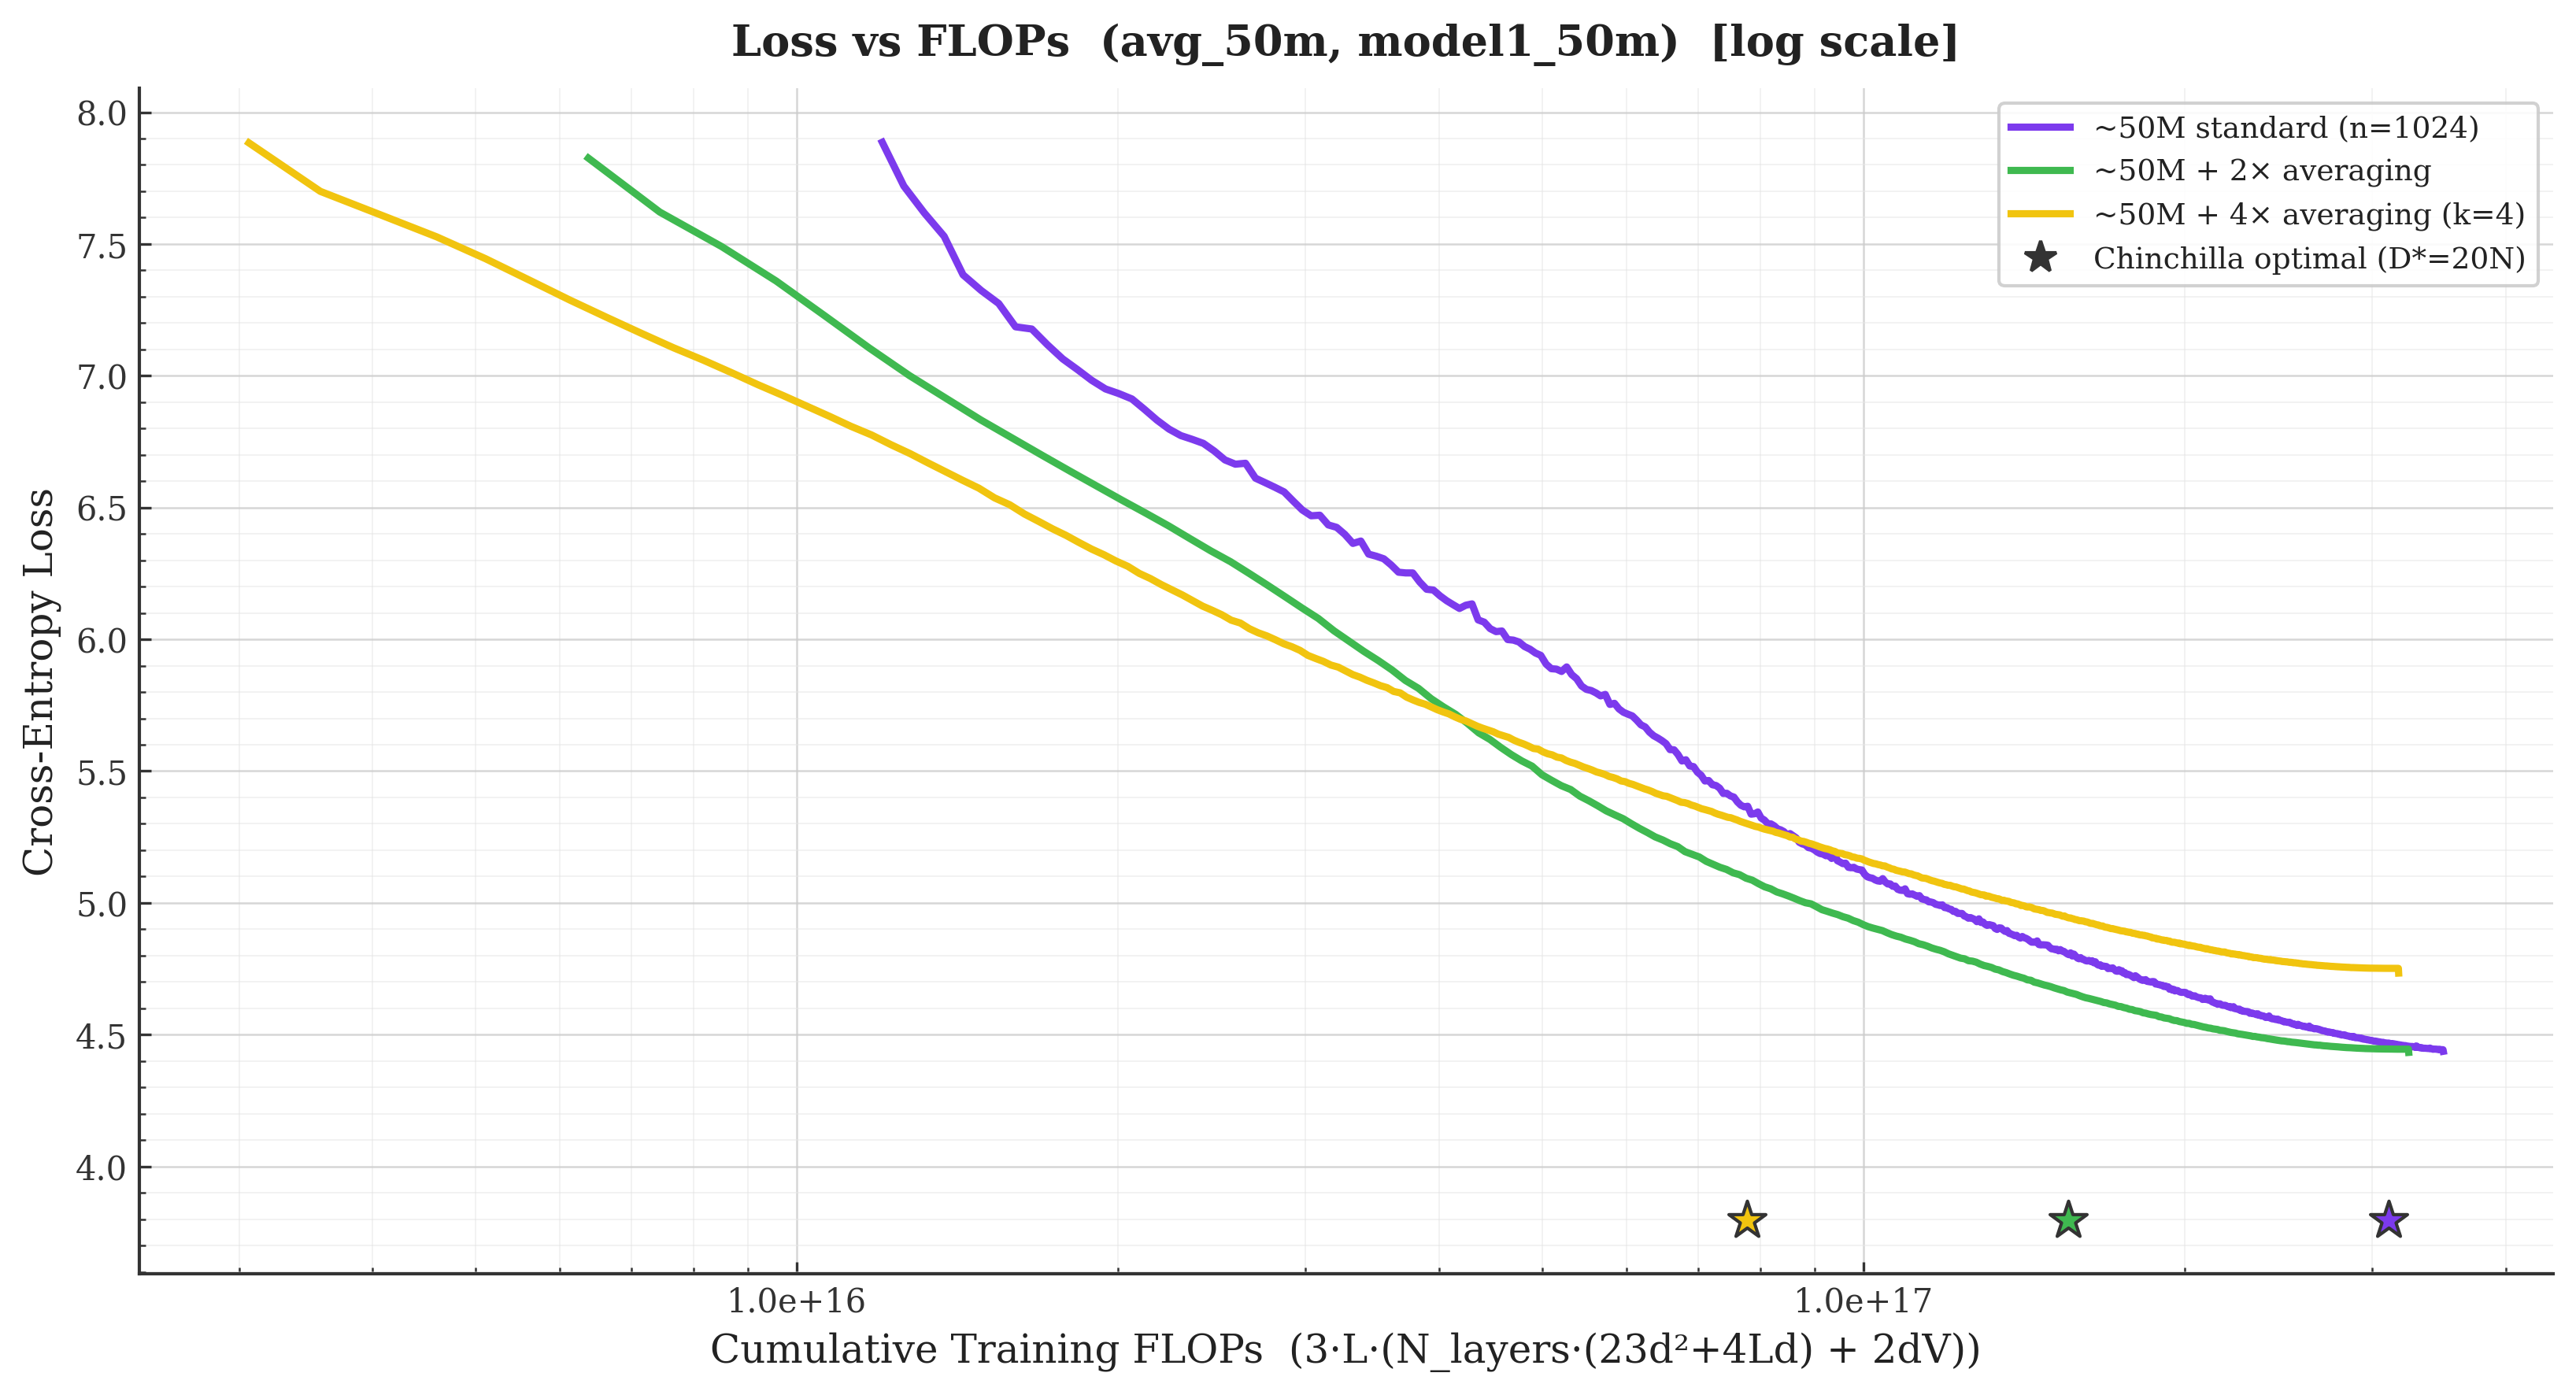
\includegraphics[height=0.70\textheight,keepaspectratio]{50m_loss_vs_flops_log.png}

  \vspace{-0.3em}
  \scriptsize
  FLOPs are recomputed from raw tokens and transformer length; the CSV
  \texttt{cumulative\_flops} column is ignored.  Curves show offset-0 eval CE.
\end{frame}

\begin{frame}{$k{=}2$ pooling ablations: loss vs training FLOPs}
  \centering
  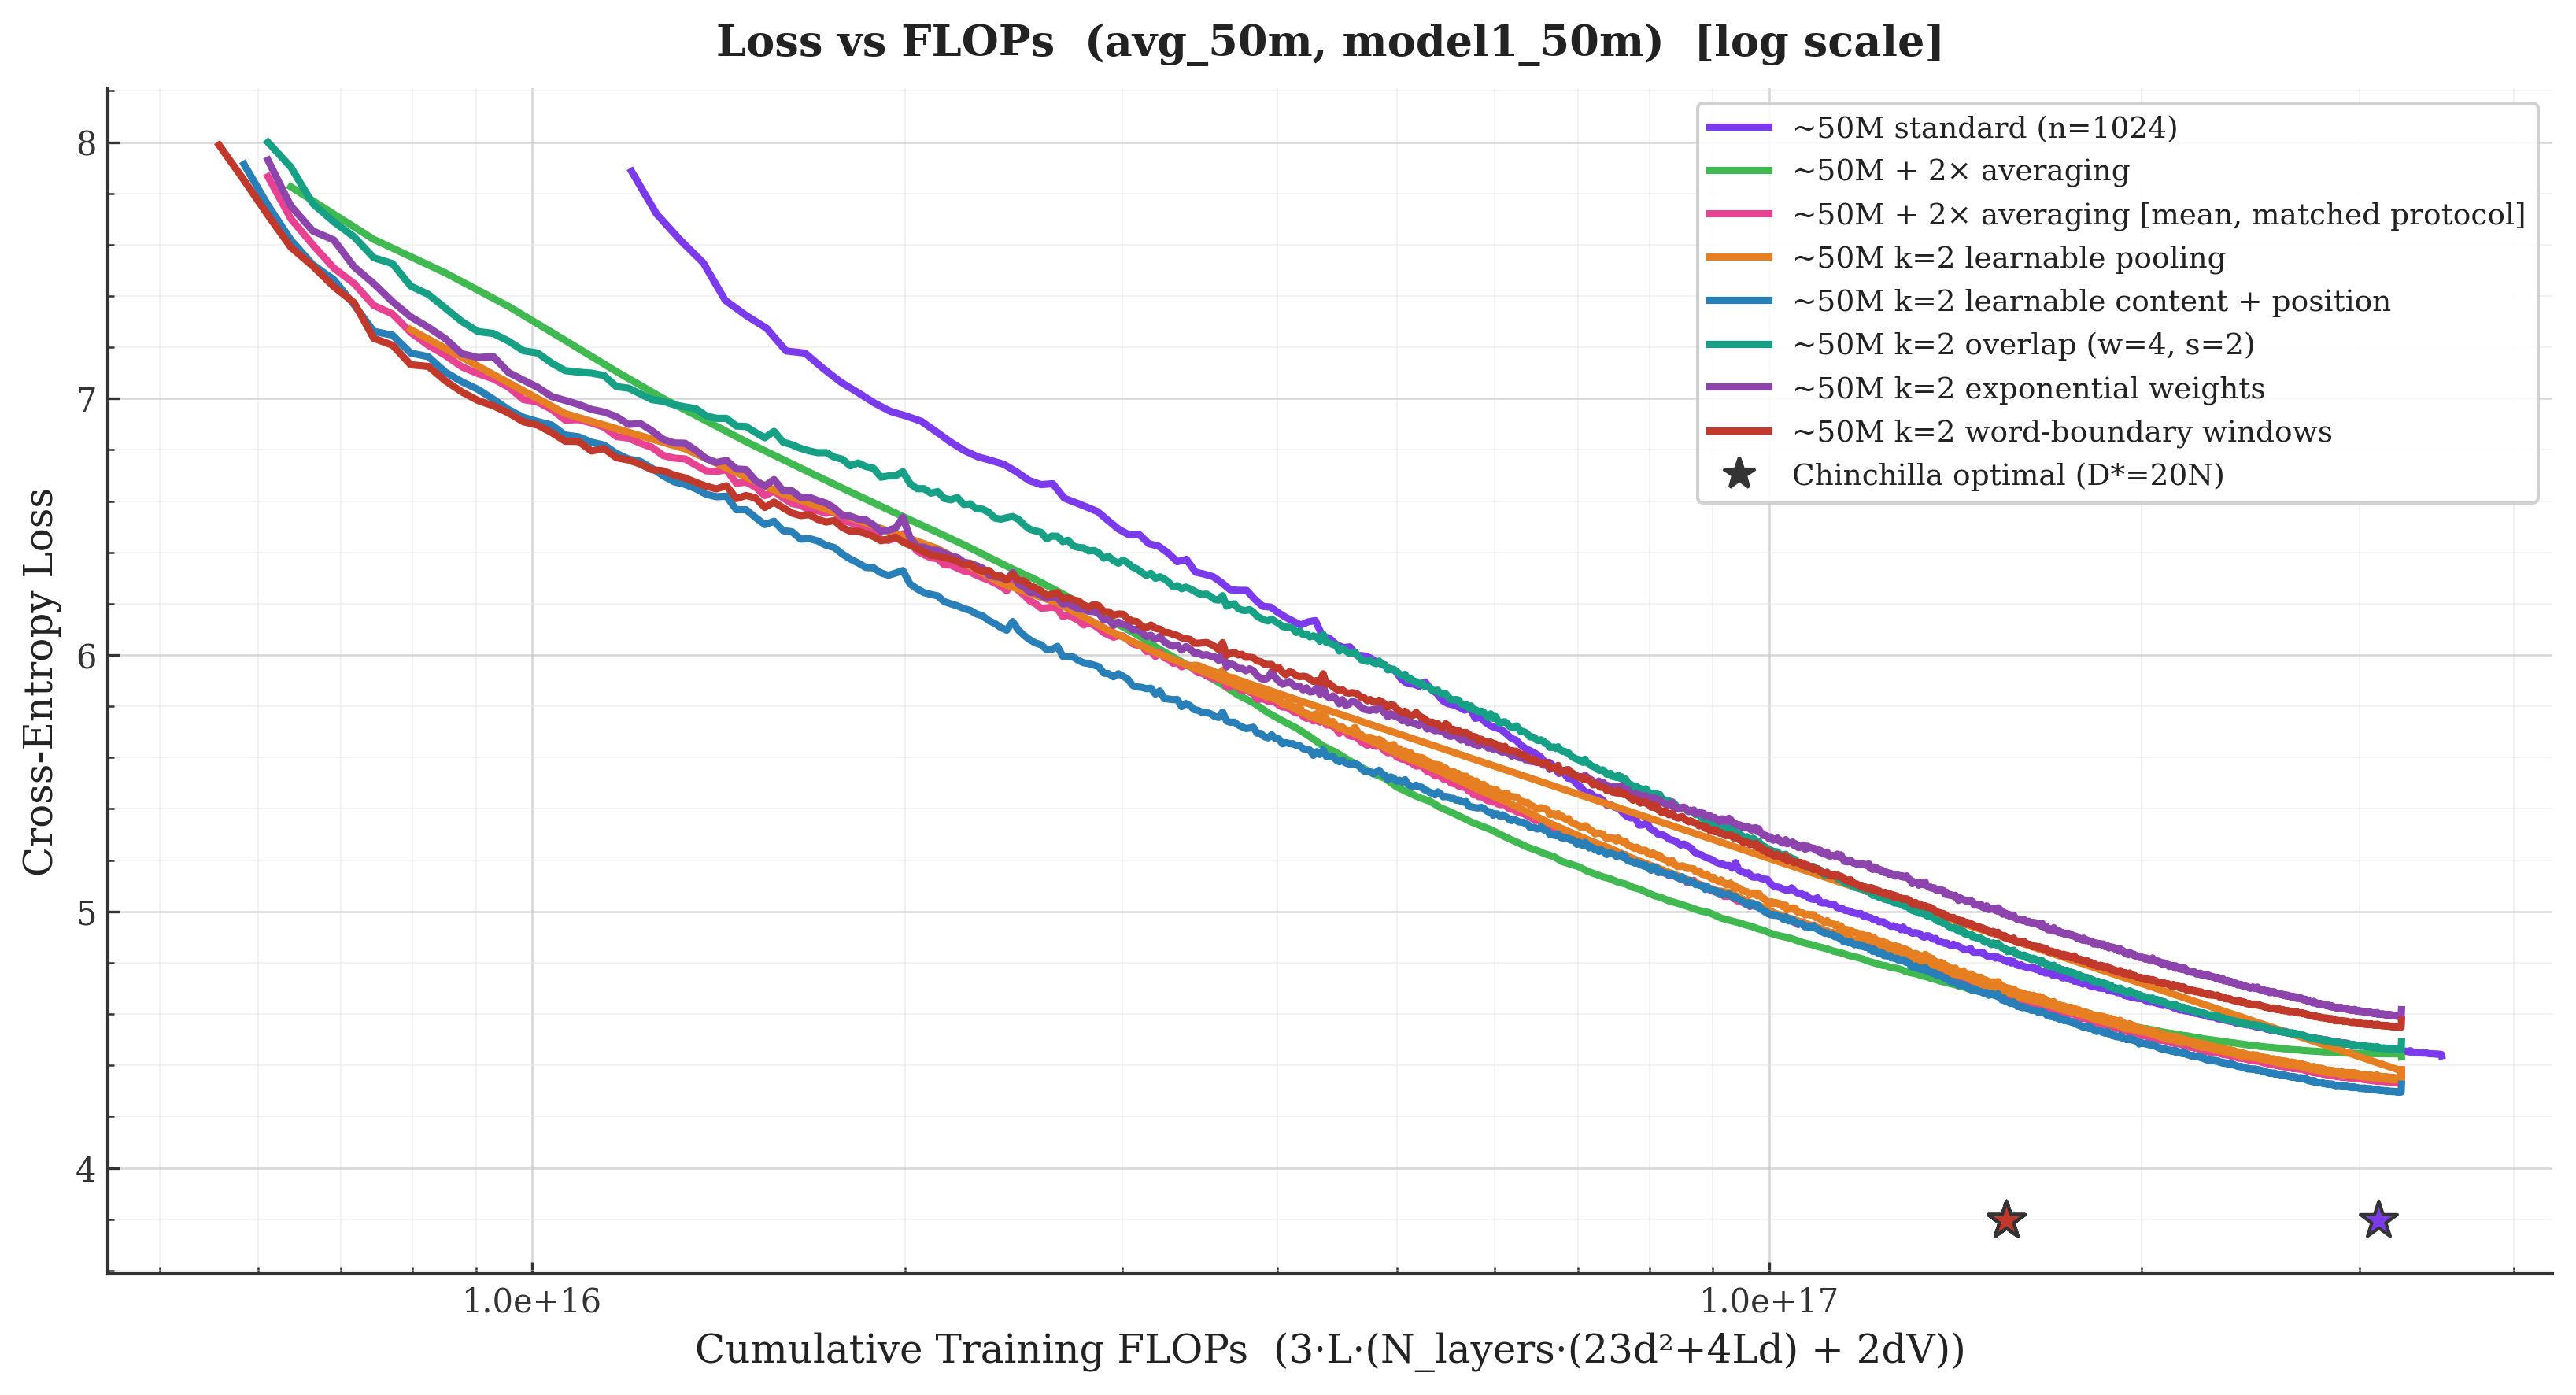
\includegraphics[height=0.70\textheight,keepaspectratio]{50m_abl_k2_loss_vs_flops_log.png}

  \vspace{-0.3em}
  \scriptsize
  All $k{=}2$ variants at 2.00B raw tokens under the matched protocol
  (old-protocol mean shown for reference). Learnable + position and matched
  mean track each other closely; the gap opens late in training.
\end{frame}

\begin{frame}{$k{=}4$ pooling ablations: loss vs training FLOPs}
  \centering
  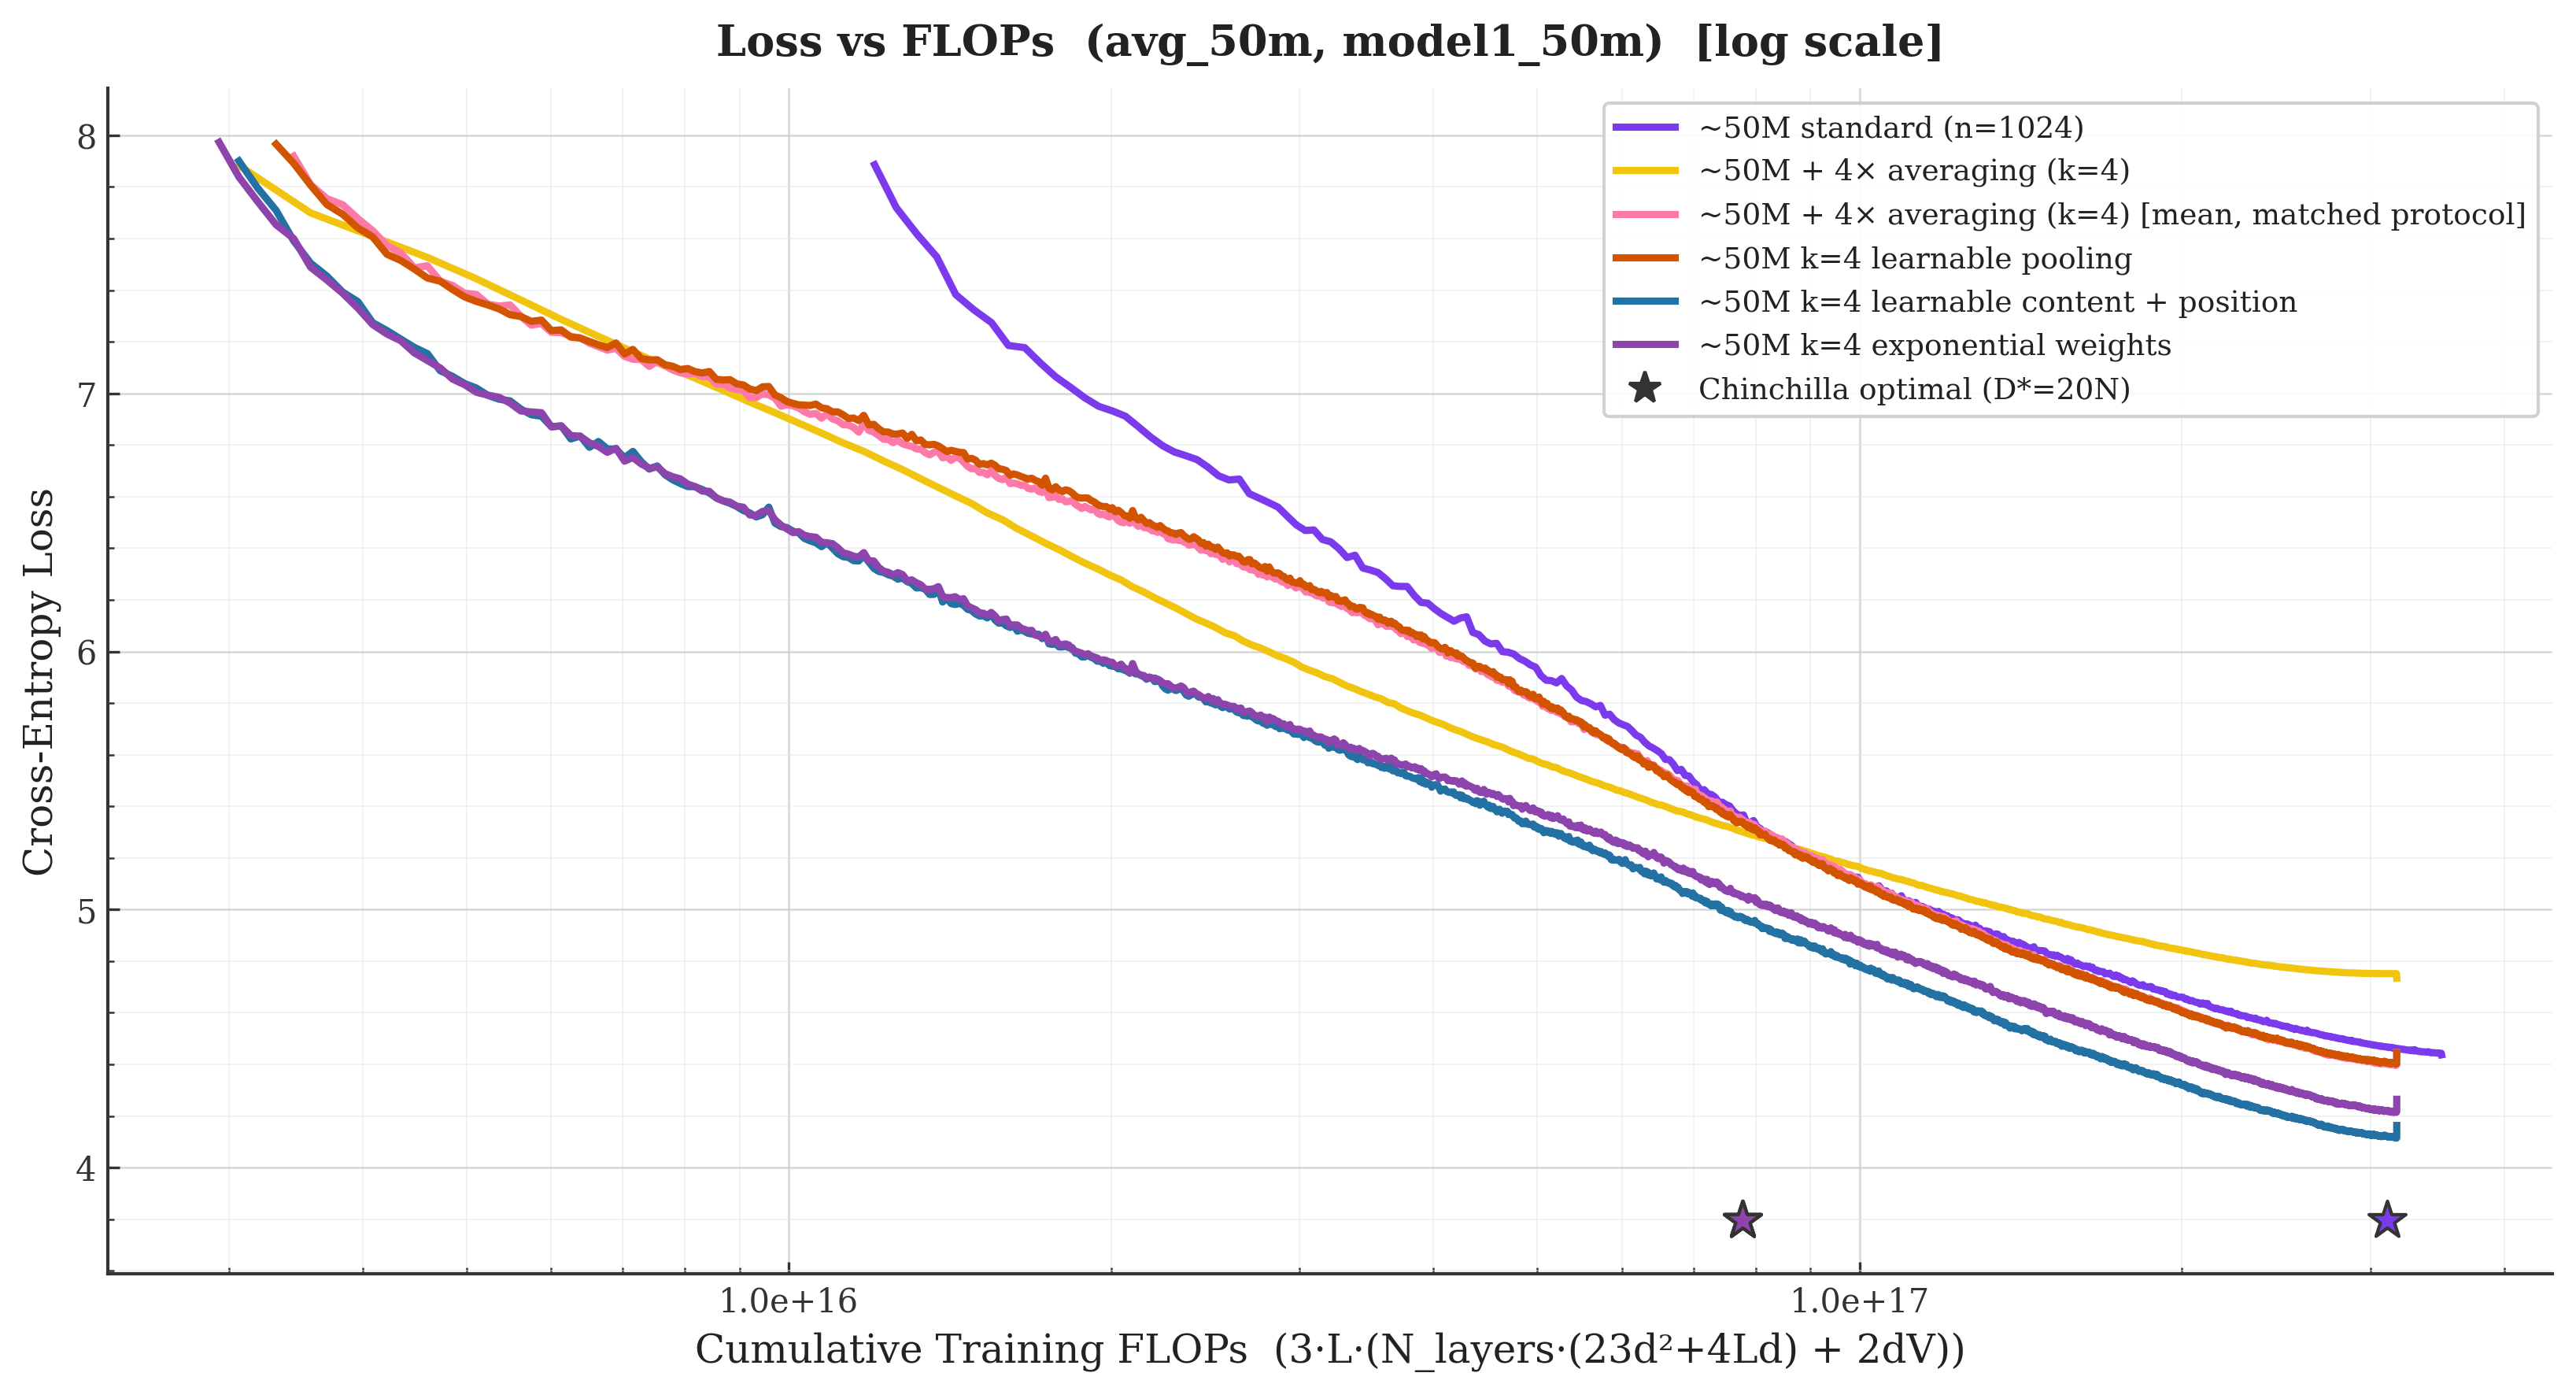
\includegraphics[height=0.70\textheight,keepaspectratio]{50m_abl_k4_loss_vs_flops_log.png}

  \vspace{-0.3em}
  \scriptsize
  All $k{=}4$ variants at 4.07B raw tokens under the matched protocol
  (old-protocol mean shown for reference). The positional-prior methods
  (learnable + position, exponential) separate from the position-blind ones
  (mean, content-only learnable) early and stay ahead.
\end{frame}

\begin{frame}{Pooling ablations: combined results ($k{=}2$ and $k{=}4$)}
  \small
  \begin{center}
  \begin{tabular}{lcccc}
    \toprule
    & \multicolumn{2}{c}{$k{=}2$ (2.00B)} & \multicolumn{2}{c}{$k{=}4$ (4.07B)} \\
    \cmidrule(lr){2-3}\cmidrule(lr){4-5}
    Pooling & Final CE & PPL & Final CE & PPL \\
    \midrule
    \good{\textbf{Learnable + position}} & \good{\textbf{4.326}} & \good{\textbf{75.7}}
      & \good{\textbf{4.163}} & \good{\textbf{64.3}} \\
    Mean (matched rerun) & 4.363 & 78.5 & 4.446 & 85.2 \\
    Learnable (content only) & 4.383 & 80.1 & 4.445 & 85.2 \\
    Exponential (fixed) & 4.617 & 101.2 & 4.265 & 71.1 \\
    Overlap ($w{=}4,s{=}2$) & 4.492 & 89.3 & -- & -- \\
    Word-aligned & 4.577 & 97.2 & -- & -- \\
    \midrule
    \textit{Mean (old protocol, ref.)} & \textit{4.433} & \textit{84.2}
      & \textit{4.734} & \textit{113.7} \\
    \bottomrule
  \end{tabular}
  \end{center}

  \vspace{0.4em}
  \begin{block}{One rule wins both regimes}
    \good{Learnable + position} is the only method that is best at
    \emph{both} compression ratios. Every other rule is regime-specific:
    mean is second at $k{=}2$ but poor at $k{=}4$; exponential is second at
    $k{=}4$ but worst at $k{=}2$.
  \end{block}
\end{frame}

\begin{frame}{$k{=}2$ pooling ablations: detailed results (now fully matched)}
  \footnotesize
  \begin{center}
  \begin{tabular}{lccccc}
    \toprule
    Pooling & 25\% & 50\% & 75\% & Final & Final PPL \\
    \midrule
    \good{\textbf{Learnable + position}} & \good{5.170} & \good{4.619} &
      \good{4.389} & \good{\textbf{4.326}} & \good{75.7} \\
    Mean (matched rerun) & 5.174 & 4.649 & 4.425 & 4.363 & 78.5 \\
    Learnable (content only) & 5.222 & 4.675 & 4.443 & 4.383 & 80.1 \\
    Overlap ($w{=}4,s{=}2$) & 5.460 & 4.820 & 4.562 & 4.492 & 89.3 \\
    Word-aligned & 5.413 & 4.872 & 4.640 & 4.577 & 97.2 \\
    Exponential & 5.439 & 4.962 & 4.707 & 4.617 & 101.2 \\
    \midrule
    \textit{Mean (old protocol, ref.)} & \textit{5.061} & \textit{4.638}
      & \textit{4.480} & \textit{4.433} & \textit{84.2} \\
    \bottomrule
  \end{tabular}
  \end{center}

  \vspace{0.3em}
  \begin{itemize}
    \item \good{Learnable + position is the best rule}: $0.037$ nats ahead of
          matched mean at the endpoint, and ahead at every checkpoint
    \item \bad{Revision of last time's conclusion:} with the matched mean
          control in place, \textbf{content-only learnable no longer beats
          mean} (4.383 vs 4.363) --- its earlier lead was the update-schedule
          confound
    \item Matched mean (4.363) vs old-protocol mean (4.433): the protocol
          alone is worth $0.070$ nats at $k{=}2$
    \item Recency bias, overlap, and word alignment all remain worse than
          plain mean under matched conditions
  \end{itemize}

  \vspace{0.1em}
  \scriptsize All six runs above the rule share the same token budget (2.00B)
  and training schedule; checkpoints at 25/50/75/100\%.
\end{frame}

\begin{frame}{$k{=}4$ pooling ablations: position matters, and content adds on top}
  \footnotesize
  \begin{center}
  \begin{tabular}{lccccc}
    \toprule
    Pooling & 25\% & 50\% & 75\% & Final & Final PPL \\
    \midrule
    \good{\textbf{Learnable + position}} & \good{4.951} & \good{4.463} &
      \good{4.224} & \good{\textbf{4.163}} & \good{64.3} \\
    Exponential (fixed) & 5.041 & 4.569 & 4.330 & 4.265 & 71.1 \\
    Mean (matched rerun) & 5.326 & 4.756 & 4.505 & 4.446 & 85.2 \\
    Learnable (content only) & 5.315 & 4.753 & 4.512 & 4.445 & 85.2 \\
    \midrule
    \textit{Mean (old protocol, ref.)} & \textit{5.290} & \textit{4.934}
      & \textit{4.786} & \textit{4.734} & \textit{113.7} \\
    \bottomrule
  \end{tabular}
  \end{center}

  \vspace{0.4em}
  \begin{itemize}
    \item \good{Learnable + position wins at every checkpoint}: $0.102$ nats
          below exponential at the endpoint (PPL 64.3 vs 71.1) --- initialized
          at the exponential profile, then content adapts on top
    \item The recency prior is confirmed against a \textbf{matched} mean
          control now: exponential beats matched mean by $0.181$ nats
    \item Content-only learnable lands exactly on matched mean
          (4.445 vs 4.446): a position-blind scorer adds \emph{nothing} at
          $k{=}4$ --- position was the missing ingredient all along
    \item Matched mean (4.446) vs old-protocol mean (4.734): the update
          schedule alone is worth $0.288$ nats at $k{=}4$
  \end{itemize}
\end{frame}

\begin{frame}{Why does learned pooling lose to fixed weights at $k{=}4$?}
  \footnotesize
  The content-only learnable pooler is deliberately small:
  \[
    s_i = w^\top e_i+b,\qquad
    \alpha_i=\operatorname{softmax}(s_i),\qquad
    \bar e=\sum_{i=1}^{k}\alpha_i e_i .
  \]

  \begin{itemize}
    \item The scorer sees each token embedding independently, \emph{before} the
          transformer and before positional information is added
    \item It is therefore \textbf{content-aware but position-blind}: the same
          token receives the same score whether it is first or last in a window
    \item Exponential pooling supplies the missing inductive bias directly:
          later tokens always receive more weight
    \item At $k{=}2$, this prior is too aggressive; at $k{=}4$, avoiding equal
          dilution matters enough that the recency prior wins decisively
  \end{itemize}

  \begin{block}{Mechanism ablation: done, and it confirms the story}
    We added a learned positional bias, $s_i=w^\top e_i+b+p_i$, with $p_i$
    initialized at uniform ($k{=}2$) / the exponential profile ($k{=}4$).
    Result: \good{best rule at both $k$} (4.326 at $k{=}2$; 4.163 at $k{=}4$).
    The content-only scorer ties matched mean at $k{=}4$ (4.445 vs 4.446), so
    position was the missing ingredient; content then adds a further
    $0.102$ nats on top of the fixed prior. Next: inspect the learned
    $\alpha_i$ by position and token type.
  \end{block}
\end{frame}

\begin{frame}{Learnable + position pooling: definition}
  For a window of $k$ embeddings $e_1, \dots, e_k$, the pooler scores each
  slot with a shared content term plus a learned per-slot bias:
  \[
    s_i = w^\top e_i + b + p_i,\qquad
    \alpha = \operatorname{softmax}(s_1, \dots, s_k),\qquad
    \bar e = \sum_{i=1}^{k} \alpha_i\, e_i .
  \]

  \vspace{0.3em}
  \small
  \begin{itemize}
    \item \textbf{Parameters:} $w \in \mathbb{R}^{d}$, $b \in \mathbb{R}$,
          $p \in \mathbb{R}^{k}$ $\Rightarrow$ $d + 1 + k$ total
          (515 at $k{=}2$, 517 at $k{=}4$ for $d{=}512$) --- negligible vs
          the 50M backbone
    \item \textbf{Initialization at the best fixed rule of each regime:}
          $w = 0$, $b = 0$ always; $p = 0$ at $k{=}2$ (starts exactly at
          \emph{mean} pooling) and $p_i \propto \ln$-spaced exponential
          profile (last/first weight ratio 20) at $k{=}4$ (starts exactly at
          \emph{exponential} pooling)
    \item \textbf{Decomposition by construction:} $p_i$ carries the
          positional prior the content-only scorer cannot express
          ($s_i = w^\top e_i + b$ is position-blind); $w^\top e_i$ adds
          content adaptation on top
    \item Trained end-to-end with the ordinary LM loss; no auxiliary
          objective
  \end{itemize}
\end{frame}

\begin{frame}{What can we conclude from the pooling sweep?}
  \begin{columns}[T]
    \column{0.49\textwidth}
    \textbf{\good{Supported by fully matched runs}}
    \begin{itemize}
      \item \good{Learnable + position is the best rule at both $k$}
            ($-0.037$ vs mean at $k{=}2$; $-0.283$ at $k{=}4$)
      \item Content-only learnable does \emph{not} beat matched mean
            (its earlier lead was the protocol confound)
      \item At $k{=}4$ the positional prior does the heavy lifting
            ($-0.181$ nats); content adds $-0.102$ more
      \item Overlap, word alignment, and pure recency all lose to plain
            mean at $k{=}2$
      \item Optimal pooling is \textbf{$k$-dependent}; the hybrid subsumes
            both regimes
    \end{itemize}

    \column{0.49\textwidth}
    \textbf{Mechanism picture (now supported)}
    \begin{itemize}
      \item Small $k$: both tokens carry signal; near-uniform weights plus
            mild content adaptation win
      \item Large $k$: the window's last token is the predictive one; an
            explicit positional prior preserves it, and a position-blind
            scorer cannot learn this
      \item Pooling controls which information survives before attention
            begins --- worth $0.28$ nats at $k{=}4$ for 517 parameters
      \item Protocol effect is large ($0.07$--$0.29$ nats): matched controls
            were essential
    \end{itemize}
  \end{columns}

\end{frame}

\begin{frame}{Pooling ablations: control status}
  \small
  \begin{block}{\good{Done: matched mean controls}}
    Mean $k{=}2$ and $k{=}4$ have been rerun under the exact ablation protocol
    (batch, update count, warmup exposure, tied embeddings, eval batches).
    Every pooling comparison on the previous slides is now within one matched
    protocol. The protocol itself moves mean by $0.070$ nats at $k{=}2$ and
    $0.288$ at $k{=}4$, which retroactively explains why content-only
    learnable seemed to beat mean last time.
  \end{block}

  \begin{itemize}
    \item \textbf{Still open --- seeds:} single run per variant; 2--3 seeds
          for learnable+pos and matched mean would put error bars on the
          $0.037$-nat $k{=}2$ gap (the $k{=}4$ gaps are large enough to be
          safe)
    \item \textbf{Still open --- metric:} curves report offset-0 loss;
          full-position offset-ensemble NLL rescoring is queued
    \item \textbf{Still open --- word method:} variable compression and
          word-start targets change the prediction distribution; needs
          bits-per-byte rescoring
    \item \good{\textbf{Done --- $k{=}1$ update-count control}} at fixed
          FLOPs: the control \bad{beats every $k{=}2$ variant} (4.142 vs
          4.326 best) --- see the update-count control slides
  \end{itemize}

  \tiny Data hygiene: clean the duplicated/malformed learnable-$k{=}2$
  log before publication plotting (the two recorded endpoints agree:
  4.379 vs 4.383).
\end{frame}

% =====================================================================
\section{Plan}
% =====================================================================

\begin{frame}{Plan 1: scaling --- 500M is in, and the decay reached zero}
  \small
  \textbf{Question (revised):} does averaging beat an \emph{update-matched}
  baseline at any scale?
  \begin{itemize}
    \item Multipliers vs the batch-16 baselines: $1.58\times$ (50M) $\to$
          $1.44\times$ (125M) $\to$ $1.32\times$ (250M) $\to$
          \bad{500M: gap crosses zero on the native metric} --- shrinking,
          as projected
    \item At 50M the update-count control flips the result outright
          (4.142 vs 4.326 for the best $k{=}2$); the 500M result is
          independent evidence pointing the same direction
    \item \textbf{Still open, now higher priority:} the same $k{=}1$
          half-batch control at 125M/250M/500M, and seed replicates at 500M
          to know whether the crossover is real or a single unlucky seed
    \item 1B is no longer an obvious next spend until we know whether 500M's
          near-zero gap is signal or noise
  \end{itemize}

  \vspace{0.4em}
  Deliverable unchanged: Chinchilla-style $L(C)$ fits per family, but on
  update-matched pairs.

  \vspace{0.4em}
  \begin{alertblock}{Logistics}
    \begin{itemize}
      \item $k{=}2$ consumes $2\times$ raw data: 250M $k{=}2$ (10B) already
            exhausts FineWeb sample-10BT $\Rightarrow$ $\geq$100BT slice
            before 500M/1B
      \item Standardize on offset-ensemble NLL as the reported metric
    \end{itemize}
  \end{alertblock}
\end{frame}

\begin{frame}{Plan 2: consequences of the Config B result}
  \textbf{Config A becomes the paper's configuration.} Scaling runs
  (250M/500M/1B) proceed with seq\_len fixed, transformer length $=$ seq/$k$.

  \vspace{0.5em}
  \textbf{Config B becomes an ablation}, and a useful one: it shows the
  Config A gains are \emph{not} a context effect --- and the full-attention
  control shows the context failure is method-independent.

  \vspace{0.5em}
  \textbf{The context-for-context result is a keeper:} same loss as full
  attention at $1.26\times$ less training compute and half the inference KV
  cache. If long context matters for an application, averaging is the cheaper
  route --- worth demonstrating on data where context actually helps.

  \vspace{0.5em}
  \textbf{Follow-ups to make the context conclusion airtight:}
  \begin{itemize}
    \item Loss-vs-position curves (Config B $k{=}2$ and full-attention
          $k{=}1$): does loss improve at positions with $>$1024 tokens of
          available context?
    \item Document-length distribution of FineWeb (most docs $<$ 1024 tokens)
    \item Long-document data (PG19, code) and/or document-boundary attention
          masking --- the setting where the $1.26\times$ advantage would
          translate into a headline long-context result
  \end{itemize}
\end{frame}

\begin{frame}{Plan 3: remaining controls after the pooling sweep}
  \small
  \begin{columns}[T]
    \column{0.5\textwidth}
    \textbf{Controls}
    \begin{itemize}
      \item \good{[done]} Mean $k{=}2/k{=}4$ matched reruns
      \item \good{[done]} Learnable + position at both $k$ (best rule at
            both)
      \item Full-position offset-ensemble NLL for every pooling rule
      \item 2--3 seeds for learnable+pos and matched mean (the $k{=}2$ gap
            is only $0.037$ nats)
      \item \good{[done]} $k{=}1$ update-count control --- control wins;
            repeat at 125M/250M
      \item Coarser-tokenizer baseline ($\sim\!2\times$ mean token length),
            compared in bits-per-byte
    \end{itemize}

    \column{0.5\textwidth}
    \textbf{Method follow-ups}
    \begin{itemize}
      \item Inspect learnable+pos weights: learned $\alpha_i$ by position
            and token type; position-wise loss
      \item Promote learnable+pos to the scaling runs? (517 params, best at
            both $k$) --- decide before 500M
      \item Add strided subsampling as an information-content control
      \item Clean $k \in \{2,4,8\}$ sweep under one training protocol
      \item Small local decoder to emit all $k$ tokens (Block-Transformer
            style) $\Rightarrow$ native generation + downstream zero-shot
            evals (LAMBADA, HellaSwag, PIQA, ARC-E)
    \end{itemize}
  \end{columns}
\end{frame}

\begin{frame}{Positioning: closest prior work}
  \textbf{Patch-Level Training for LLMs} (Shao et al., 2024; ICLR'25) ---
  nearly the same mechanism: average $K$ token embeddings, predict the next
  patch, then \emph{fine-tune at token level}. 370M--2.7B, claims
  $0.5\times$ cost.

  \vspace{0.4em}
  \textbf{Our deltas (to sharpen):}
  \begin{itemize}
    \item Patch-level as the \emph{final operating point}, not a warm-up ---
          made viable by the offset-ensemble eval + rotating-offset generation
    \item FLOP-controlled \emph{scaling-law} treatment (efficiency vs scale),
          not single budget points
    \item Context-extension angle (Config B): same positions, double context,
          half the inference KV cost
  \end{itemize}

  \vspace{0.4em}
  \small Also related: MegaByte, Byte Latent Transformer (dynamic patches),
  Block Transformer, Funnel/Hourglass, multi-token prediction
  (Gloeckle et al.; DeepSeek-V3 MTP), context compression (gist tokens,
  AutoCompressor, ICAE).
\end{frame}

\begin{frame}{Summary / discussion}
  \scriptsize
  \begin{itemize}
    \item Vs batch-16 baselines, averaging wins at 50M/125M/250M: $-3.4\%$
          perplexity at $0.91\times$ FLOPs on the full-coverage metric at
          125M; equal-loss savings $1.58\times$ (50M), $1.44\times$ (125M),
          $1.32\times$ (250M) --- but the multiplier \bad{shrinks} with scale
    \item \bad{At 500M the gap crosses zero}: native loss slightly
          \emph{favors the baseline} ($-0.003$), full-position still barely
          favors averaging ($+0.003$) --- both far below our $0.070$-nat
          noise floor, and the same direction as the update-count control
    \item \bad{The 50M update-count control flips the headline}: a $k{=}1$
          baseline with matched updates and positions beats every $k{=}2$
          variant (4.142 vs 4.326 best) at comparable FLOPs. Update schedule
          alone is worth $-0.295$ nats; the $k{=}2$ edge was $-0.074$
    \item Evaluation gap closed with offset-ensemble NLL --- retroactively
          valid, and it unlocks generation
    \item Mechanism decomposed: the gain vs batch-16 baselines is
          \textbf{data-per-FLOP, not context} --- extended context loses at
          50M \emph{by any method} ($+0.21$ nats for both $k{=}2$ averaging
          and $k{=}1$ full attention)
    \item Context-for-context: averaging \good{matches full attention at 2048
          context with $1.26\times$ less compute} and half the inference KV
          cache
    \item Pooling sweep, now with matched mean controls:
          \good{learnable + position is the best rule at both $k$}
          ($-0.037$ nats vs mean at $k{=}2$, $-0.283$ at $k{=}4$);
          content-only learnable ties mean, so position is the key
          ingredient at $k{=}4$
    \item Remaining pooling caveats: single seed per variant, offset-0
          metric (full-position rescoring queued)
  \end{itemize}
\end{frame}

\begin{frame}{Questions for discussion}
  \textbf{Questions for discussion}
  \begin{itemize}
    \item The 500M gap is within noise and we have one seed: is it worth
          2--3 seed replicates at 500M before deciding whether to spend on
          1B, or do we treat the crossover as decisive on its own?
    \item The update-count control at 50M reverses the headline: run the
          same control at 125M/250M/500M first, or also give $k{=}2$ the
          half-batch treatment to test whether small-batch gains are
          symmetric?
    \item If averaging loses update-matched everywhere: is
          context-for-context (same loss, half the KV cache) plus the
          pooling findings a sufficient paper, or does the project pivot?
    \item Promote learnable + position pooling to any remaining scaling
          runs, or keep the scaling story on parameter-free mean pooling?
    \item Is the context negative result worth a deeper treatment
          (loss-vs-position, long-document data) or one ablation slide?
  \end{itemize}
\end{frame}

\end{document}
